% This is the Reed College LaTeX thesis template. Most of the work
% for the document class was done by Sam Noble (SN), as well as this
% template. Later comments etc. by Ben Salzberg (BTS). Additional
% restructuring and APA support by Jess Youngberg (JY).
% Your comments and suggestions are more than welcome; please email
% them to cus@reed.edu
%
% See http://web.reed.edu/cis/help/latex.html for help. There are a
% great bunch of help pages there, with notes on
% getting started, bibtex, etc. Go there and read it if you're not
% already familiar with LaTeX.
%
% Any line that starts with a percent symbol is a comment.
% They won't show up in the document, and are useful for notes
% to yourself and explaining commands.
% Commenting also removes a line from the document;
% very handy for troubleshooting problems. -BTS

% As far as I know, this follows the requirements laid out in
% the 2002-2003 Senior Handbook. Ask a librarian to check the
% document before binding. -SN

%%
%% Preamble
%%
% \documentclass{<something>} must begin each LaTeX document
\documentclass[12pt,twoside]{reedthesis}
% Packages are extensions to the basic LaTeX functions. Whatever you
% want to typeset, there is probably a package out there for it.
% Chemistry (chemtex), screenplays, you name it.
% Check out CTAN to see: http://www.ctan.org/
%%
\usepackage{graphicx,latexsym}
\usepackage{amssymb,amsthm,amsmath}
\usepackage{longtable,booktabs,setspace}
\usepackage{chemarr} %% Useful for one reaction arrow, useless if you're not a chem major
\usepackage[hyphens]{url}
\usepackage{rotating}
\usepackage{natbib}
\usepackage{listings}
\usepackage{tikz}
\usepackage{xcolor,colortbl}
\usepackage{float}
\usepackage{algorithm}
\usepackage[noend]{algpseudocode}
\usepackage{subcaption}
%\usepackage[english]{babel}
%\usepackage[autostyle]{csquotes}



\newenvironment{codeexample}[1][htb]
{\floatname{algorithm}{Code Example}%\renewcommand{\algorithmcfname}{Code example}% Update algorithm name
	\begin{algorithm}[#1]%
	}{\end{algorithm}}


\lstset
{ %Formatting for code in appendix
	basicstyle=\footnotesize,
	numbers=left,
	stepnumber=1,
	showstringspaces=false,
	tabsize=4,
	breaklines=true,
	breakatwhitespace=false,
}

% Comment out the natbib line above and uncomment the following two lines to use the new
% biblatex-chicago style, for Chicago A. Also make some changes at the end where the
% bibliography is included.
%\usepackage{biblatex-chicago}
%\bibliography{thesis}

% \usepackage{times} % other fonts are available like times, bookman, charter, palatino

\newcommand{\ceil}[1]{\lceil #1 \rceil}
\newcommand{\floor}[1]{\lfloor #1 \rfloor}



\title{Efficient Parallelism Detection for Heterogeneous Computing}
\author{Benjamin Black}
% The month and year that you submit your FINAL draft TO THE LIBRARY (May or December)
\date{May 2018}
\division{Mathematics and Natural Sciences}
\advisor{Kelly Shaw}
%If you have two advisors for some reason, you can use the following
%\altadvisor{Your Other Advisor}
%%% Remember to use the correct department!
\department{Mathematics}
% if you're writing a thesis in an interdisciplinary major,
% uncomment the line below and change the text as appropriate.
% check the Senior Handbook if unsure.
%\thedivisionof{The Established Interdisciplinary Committee for}
% if you want the approval page to say "Approved for the Committee",
% uncomment the next line
%\approvedforthe{Committee}

\setlength{\parskip}{0pt}
%%
%% End Preamble
%%
%% The fun begins:
\begin{document}

  \maketitle
  \frontmatter % this stuff will be roman-numbered
  \pagestyle{empty} % this removes page numbers from the frontmatter

% Acknowledgements (Acceptable American spelling) are optional
% So are Acknowledgments (proper English spelling)
    %\chapter*{Acknowledgments}
	%I want to thank a few people.

% The preface is optional
% To remove it, comment it out or delete it.
    %\chapter*{Preface}
	%This is an example of a thesis setup to use the reed thesis document class.

%
%
%    \chapter*{List of Abbreviations}
%		You can always change the way your abbreviations are formatted. Play around with it yourself, use tables, or come to CUS if you'd like to change the way it looks. You can also completely remove this chapter if you have no need for a list of abbreviations. Here is an example of what this could look like:
%
%	\begin{table}[h]
%	\centering % You could remove this to move table to the left
%	\begin{tabular}{ll}
%		\textbf{ABC}  	&  American Broadcasting Company \\
%		\textbf{CBS}  	&  Columbia Broadcasting System\\
%		\textbf{CDC}  	&  Center for Disease Control \\
%		\textbf{CIA}  	&  Central Intelligence Agency\\
%		\textbf{CLBR} 	&  Center for Life Beyond Reed\\
%		\textbf{CUS}  	&  Computer User Services\\
%		\textbf{FBI}  	&  Federal Bureau of Investigation\\
%		\textbf{NBC}  	&  National Broadcasting Corporation\\
%	\end{tabular}
%	\end{table}
%

    \tableofcontents
% if you want a list of tables, optional
    \listoftables
% if you want a list of figures, also optional
    \listoffigures

% The abstract is not required if you're writing a creative thesis (but aren't they all?)
% If your abstract is longer than a page, there may be a formatting issue.
    \chapter*{Abstract}
	
	We are in the era of heterogeneous computing, where applications need to use more than one type of processor in order to improve performance. But programmers are not always taught how to best use these new processors, which results in poor use of hardware, lost performance, and lost power savings. One challenge for the programmer is that these new processors often rely on software to define parallel execution of code; unfortunately, programmers often have limited experience dealing with the problems associated with writing parallel applications. To help the programmer, we suggest building a tool that combines results from dynamic parallelism detection and workload characterization. For parallelism detection, we built a tool which detects whether parallelism exists in loops, and if not, determines why it does not. We confirm prior work that the naive implementation of the tool is memory intensive, so we implement two different methods of reducing memory consumption, one based on stride compression as introduced by SD$^3$. We find that combined with loop iteration size and variance data, this tool can be effective in guiding the programmer's parallelization efforts. %We then 
	We gather workload characterization metrics that could be combined with the parallelism information to make the tool useful in distinguishing between code that is effective on GPUs vs. CPUs, but we did not make use of these metrics due to time limitations. 
	
	% and one based on bit compression. the trade-offs of parallelizing their code on CPUs and GPUs, we built a tool which detects parallelism 

	
	%creates confusion and risk 

	%The preface pretty much says it all.

  \mainmatter % here the regular arabic numbering starts
  \pagestyle{fancyplain} % turns page numbering back on

%The \introduction command is provided as a convenience.
%if you want special chapter formatting, you'll probably want to avoid using it altogether

% The three lines above are to make sure that the headers are right, that the intro gets included in the table of contents, and that it doesn't get numbered 1 so that chapter one is 1.

% Double spacing: if you want to double space, or one and a half
% space, uncomment one of the following lines. You can go back to
% single spacing with the \singlespacing command.
% \onehalfspacing
% \doublespacing


\chapter*{Introduction}
\lstset{language=C++}
\addcontentsline{toc}{chapter}{Introduction}
\chaptermark{Introduction}
\markboth{Introduction}{Introduction}


		Traditional general purpose processors are designed to be easy to program while being as fast as possible at many different computation tasks. This allows the vast majority of applications to use general purpose processors exclusively. 
		
		For a long time, computer hardware tried to make the standard model of computation as fast as possible, inventing various methods such as instruction level parallelism that allowed the programmer to think of code sequentially while in actuality the code was running in parallel.
		But these methods could not scale well and eventually, the limits of these methods were found. To keep software performance improving, hardware moved to a many-core model where several cores executed code independently. Programming languages started including multi-threading features, and software developers were forced to learn how to reason about parallel programming. 
		
		But because each core of a many-core processor needs to execute general purpose code efficiently, each core is large, complex, and power hungry, so relatively few cores can be placed on a single chip. Today, high end many-core processors typically have at most two dozen cores. 
		
		This limitation was caused by the cores being general purpose. Hardware, however, does not need to be general purpose. 
		Individual applications often have a specific type of procedure that consumes the vast majority of the computing power. For these applications, hardware developers can build an accelerator that runs that procedure very efficiently but does not run other types of code. The general purpose processor running the application can use the accelerator to compute that procedure quickly and then perform the rest of the computation itself. Encryption and decryption are commonly done with accelerators. 
		
		Some hardware takes a compromise between generality and performance. Notably, Graphics Processing Units (GPUs), originally designed to accelerate graphics in video games, have become general enough to run many types of computations, and now run many important numeric scientific calculations. 
		
		This concept of using different hardware processes to run a single application process is called heterogeneous computing. 
		The computer hardware industry is starting to put several different types of processors and accelerators are on a single chip, so heterogeneous computing is gaining increasing importance.
		
		
	\section{Challenges of heterogeneous computing}
	
		Heterogeneous computing offers many challenges for the programmer. Since the different hardware platforms have different characteristics and interfaces, different programming languages, libraries, and tools need to be used when coding for each platform. The languages and tools for accelerators are generally much less user friendly than ones for general purpose processors, and programmers are less familiar with them. %, and require some experienc. 
		%	
		This means that programmers often have to put substantial effort into porting their code to an accelerator like a GPU.
		
		Even worse, there is no guarantee that an application will run faster on an accelerator. Take a GPU as an example. Because of the overhead involved in starting up work on a GPU, GPUs execute sequential code slower than CPUs. Even if the code is massively parallel, GPUs may still be unable to execute it effectively because the application depends on certain hardware characteristics of general purpose processors that are different then on GPUs. %Programmers are often be unaware of ways to best use the hardware. %depends on features that are absent from GPUs, like efficient handling of divergent branches. 
		So when a programmer tries to parallelize an application and does not have a deep understanding of GPU architecture, they are taking a certain risk: all that extra work may be for nothing. 
		
		Since the benefits of heterogeneous computing are potentially so large, reducing the risks and making heterogeneous programming more accessible to non-experts could bring significant benefits.
		
	\section{Our solution}
	
		This thesis focuses on a small part of the larger challenge of heterogeneous computing. First, we focus our attention only on CPUs and GPUs and ignore other types of hardware. This is only because we are restricted by time, we hope that our work would easily extend to other highly programmable accelerators.% like FPGAs.
		
		%This thesis focuses on two small parts of the larger challenge of heterogeneous computing:
		
		Within this focus on CPUs and GPUs, this thesis focuses only on the identification problem: 
		
		\begin{enumerate}
			\item Determining whether certain code structures are parallel or not.
			\item If so, then determining which kind of hardware would be more appropriate: CPU or GPU. 
		\end{enumerate}
	
		We suggest creating a tool which can help programmers understand how their code might perform on a many-core processor and a GPU assuming the code was ported to a GPU. %, or whether traditional CPU multi-threading would be more appropriate. 
		%This tool would run on sequential CPU code, and would speculate about 
		Ideally, this tool would not only give results based on how the code currently is, but also give information to the programmer which would help them understand how the code could be changed to give better results on different types of hardware. 
		
		The results of this tool should allow average programmers to make better decisions and assume less risk when deciding how to allocate their time, potentially allowing them to better accelerate their applications. 
		
	\section{Related work}
	
		There are two avenues of prior work which we try to combine in order to make such a tool: workload characterization and dynamic parallelism detection. 
		
		Workload characterization measures the demands applications place on hardware resources. Che et. al. created the Rodinia benchmark, to allow researchers to do workload characterization to understand differences between GPUs and CPUs.\footnote{\cite{Che:2010}} In particular, the goal for this benchmark suite is to understand the general types of workloads and data structures that work well on GPUs. In a way, they are examining the characteristics of categories of applications, where we are trying to investigate characteristics of specific applications. Workload characterization and how it relates to our goals is described in more detail in Section \ref{s:workload-characht}. 
		
		Parallelism detection analyzes which parts of sequential code might be run in parallel. Historically, applications of parallelism detection have been limited to CPUs. 
		An example commercial application of parallelism detection is the  Intel\textsuperscript{\textregistered} Advisor. The tool tells programmers which loops in the code might be parallelized, how they might be parallelized, and if not, where the problems are that are stopping it from being parallelized. 
		Intel Advisor currently costs around \$1600 and is closed source, so we will be building our own tool similar to this one but with fewer features. 
		
	
	\section{Parts of thesis}
	
		This thesis makes several contributions:
		
		\begin{enumerate}
			\item Built a memory-efficient tool to detect parallelism in loops. 
			\item Built a tool to collect a variety of metrics for our workload characterization. %, and match these metrics with the parallelism.
			\item Analyze the possible effectiveness of these tools to distinguish between GPU and CPU oriented applications.
		\end{enumerate}
	
		Chapter 1 introduces parallelism detection and approaches to improve memory efficiency. Chapter 2 describes implementation details of the tools, and Chapter 3 presents some results on how well these tools ended up working. 
		%We hope these will make progress towards the eventual goal.
	
		
\chapter{Dynamic parallelism detection}

	\section{Introduction}
	
		We need a way of determining parallelism in order to do any useful inference on hardware compatibility. However, recall that our end goals are larger than just that. We are creating a tool that helps the programmer understand their code and helps them improve the algorithms and prototype them to perform better on different hardware without having the programmer actually deal with the hardware. Consequently, we not only want a parallelism tool that figures out which parts of the code can be parallelized or not, but we also want a tool that helps the programmer understand why code might not be parallelizable and perhaps suggests how to fix it. 
		 
		We came to the conclusion that current open-source parallelism detection tools do not meet our efficiency and accuracy requirements, and so we built our own tool which does meet our needs. 
		
		This chapter goes over the necessary background for that tool. In section 1.2, we introduce the type of parallelism we are detecting, and why it is so important. In section 1.3, we introduce dynamic analysis of loops, a prerequisite for the base algorithm. In section 1.4, we introduce the base algorithm for detecting it, and the problems with that base algorithm. In section 1.5, we go over prior work in this area and discuss how it does not suit our needs completely. 
		
	\section{Loop level parallelism}
	
		Parallelism exists in different code structures and at different levels of granularity. Programmers talk about how parallelism manifests itself in code. These include task parallelism (executing different functions in parallel) and  loop parallelism (running different parts of a loop in parallel). Computer architects talk about how different kinds of parallelism can be exploited in hardware, including instruction level parallelism, thread level parallelism, and memory level parallelism. 
		
		This thesis focuses on loop-level parallelism (LLP). This type of parallelism is common, easy to detect, scalable on massively parallel processors, and simple for programmers to reason about. 
		
		\subsection{What is Loop level parallelism?}
		
		We start by introducing some terminology. A loop is a code construct that executes the same instructions over and over on different data. A loop iteration is a single execution of the code in the loop. Two loop iterations are independent if the later iteration does not use data computed by the prior iteration. 
		
		Loop level parallelism exists when every iteration of the loop can be run independently from every other iteration. 
		
		\subsection{Examples of Loop level parallelism}
		
		Here is code that performs in-place vector-scalar multiplication on a vector \texttt{B} with \texttt{n} elements. 
		%The loop executes n times, multiplying a different element of B each time. 
		
		\begin{codeexample}
			\caption{Vector-scalar multiply}\label{vec-scal-mul}
		\begin{lstlisting}
for(int i = 0; i < n; i++){
	B[i] = B[i] * c;
}
		\end{lstlisting}
		\end{codeexample}
		
		This loop is parallelizable. In this loop, each iteration is simply the calculation of \texttt{B[i] = B[i] * c} for some \texttt{i}. Since the iteration is dependent only on the element of \texttt{B} that it also updates, any of these iterations can be executed before any other iteration. So you can compute these iterations in any order without affecting correctness, so the loop is parallelizable. 
		
		In contrast, here is code that performs a cumulative sum. 
		
		\begin{codeexample}
			\caption{Cumulative Sum}\label{cum-sum}
		\begin{lstlisting}
for(int i = 1; i < n; i++){
	B[i] = B[i-1] + A[i];
}
		\end{lstlisting}
		\end{codeexample}
		
		This loop is not parallelizable. For \texttt{i > 1}, \texttt{B[i] = B[i-1] + A[i];} cannot be computed correctly until \texttt{B[i-1]} is calculated, since \texttt{B[i-1]} is used to calculate \texttt{B[i]}. To summarize, the loop must be executed in a particular order, so it is not parallelizable. 
		
		\subsection{Importance of loop level parallelism}
		
		Loop level parallelism is important to this work for four reasons: it is common, scales well on massively parallel hardware, simple for programmers to reason about, and easy to detect. 
		
		Loop level parallelism is common and easy for programmers to reason about. 
		A large amount of work in research and tool development has been devoted to exploiting loop level parallelism. Many parallelism frameworks are focused on loop level parallelism. OpenMP is a C and C++ parallelism framework that allows programmers to parallelize loops (assuming they are parallelizable) on CPUs with a single line of code. 
		
		Loop level parallelism is easy to detect compared to other types of parallelism. Restricting ourselves to this kind of parallelism will give us a simple and fast algorithm.
		Research in automatic parallelization has been focused mostly on loops, mostly because loops are more common and easier to analyze than other parallel code structures. 
		
		Finally, parallel loops often scale well on massively parallel hardware compared to parallel tasks or recursive calls, simply because they often have a large number of iterations.
%		
%		
%		Of course, loops are very common in code. As prior work on loop parallelism has shown, a large number of these loops are parallel. 
%		
%		Loop level parallelism is part of a class of parallelism called massive parallelism. That means that if the loop is reasonably large, it can be scaled to massively parallel hardware like GPUs or other kinds of accelerators. 
%		
%		Parallelizing loops is also very simple for the programmer to reason about. With OpenMP, one can parallelize loops on CPUs with a one line directive. In lower level accelerator code, like OpenCL, it is still relatively easy to translate loops into parallel kernels, just by porting the inner part of the code to an kernel, and run it on all the iterations of the loop in parallel 
%		
%		Lastly, loop level parallelism is easy to detect. The next section will give a simple algorithm to detect this. Other kinds of massive parallelism require more sophisticated analysis. 
%		
		\section{Dynamic Analysis}
		
			There are two general methods to establish parallelism in code: static analysis and dynamic analysis. Static analysis tools parse code like compilers do, analyzing syntax trees of variable assignments and loops. They attempt to establish general properties of the code. Generally, the results of static analysis are true given any possible input. Unfortunately, as code increases in complexity and generality, it becomes impossible to derive precise results in full generality. 
			%Landi proved that static data flow analysis, which is necessary for parallelism analysis, is undecidable for languages like C\footnote{\cite{Landi:1992:USA:161494.161501}}. 
			For a complex semantic property like parallelism, static analysis returns too many false negatives to be useful for practical purposes. 
			
			Dynamic analysis tools examine running processes like an interpreter does, executing a series of instructions on a particular input, while analyzing the behavior and values of the running program. Since a dynamic analysis tool only observes the program on a particular input, it can only establish properties of the code for that specific input. Therefore, dynamic analysis can give false positives for parallelism, meaning a loop might be parallelizable on the particular input, but not on others. To reduce the number of false positives, a complex input that uses many of the features of the program and reflects production use will be more helpful than a simple, contrived input. 
			
		\subsection{Dynamic Loop Detection}\label{s:loopprof-detection}
		
		Dynamic loop level parallelism detection requires a determination of when a loop starts, ends, and iterates in a running program.
		This is a surprisingly challenging problem. 
		Loops have a clean structure in high level languages like C. It is easy for both the compiler and a human to understand what code is inside the body of a loop, and when the loop starts and ends. However, this work focuses on the dynamic analysis of loops. 
		
		Doing dynamic analysis requires us to understand the structure of loops in machine code. Even if the source code is available, there is not always a precise mapping from machine code to source code, as loops may be compiled to different machine code depending on the compiler. Loops in machine code are hard to detect, as they are implemented with ``go to'' instructions (referenced in this thesis as goto). goto instructions allow the code to jump to fixed instructions elsewhere in the code. These instructions implement various functionality like if-else blocks, while loops, and break statements, so their presence does not guarantee a loop.
		
		To demonstrate the difficulty of finding loops in machine code, here is the standard way of translating the above vector-scalar multiply loop into machine code:
		
		\begin{lstlisting}
i = 1
if i >= n goto line 8
tmp1 = B[i]
tmp1 = tmp1 * c
B[i] = tmp1
i = i + 1
goto line 2
...
		\end{lstlisting} 
		
		Note that even with a single simple loop, there are two goto statements, one for creating the loop, and one for exiting the loop. With nested loops, branches, and break statements, it quickly becomes very difficult to understand where a particular loop starts and how to know that a particular loop terminated.
		So in order to understand loops in machine code, we have to somehow separate loops out from a tangle of goto instructions. 
		
		Luckily, there is prior work for doing just this. We use LoopProf \footnote{\cite{Chen:2004}} code in order to detect the locations of loops in code. In particular, LoopProf tells us where the loop begins and the nesting structure of loops. 
		
		LoopProf uses dynamic analysis in order to determine where loops are. At a high level, it tracks a list of instructions executed in a function. When a goto jumps back to a instruction on that list, then LoopProf concludes that there was a loop, and that its second iteration just started executing. 
		
		However, the LoopProf implementation, generously provided to us by its author, did not contain all of the functionality we needed. In particular, it did not detect the precise ends of loops, which we needed for dynamic dependence analysis. Consequently, we made some additions in order to suit our needs. 
		%Unfortunately, these are technical enough and far enough away from the point of this chapter, that we will not get into more detail about this. 
		
	\section{The baseline algorithm: The pairwise method}
	
		One of the goals of this thesis is to create a tool that identifies loop level parallelism. The literature has several methods to identify this type of parallelism. A particularly simple method is the naive pairwise method. This thesis's implementation will be an optimization of the pairwise method, so the naive version will be described in detail here. 
		
		Recall that loop-level parallelism occurs when each iteration of a loop can be executed independently from every other iteration, and that independence means that one iteration does not depend on data computed by another iteration. 
		The pairwise method tracks reads and writes to memory to determine dependences. Each read is considered to be an input to the computation in the loop, and each write is an output. If one loop iteration writes to one location in memory and a later iteration reads from that same location, then that is a dependence that should be recorded as it inhibits parallelism. 
		
		There is an important difference between memory and dependencies. Memory can sometimes be reused without creating dependencies. In particular, consider a location in memory that is written to before it is read in a loop iteration. The data that was previously at that location was overwritten, so the current iteration will not depend on data at that location that was written to in previous iterations. In this case, we say the location is "killed." Reads of killed memory locations are not tracked in a given iteration.
		
		The pairwise method stores two different structures for a particular loop:
		
		\begin{itemize}
			\item history table: A table of reads and writes of previous loop iterations.
			\item pending table: A table of reads and writes of the current loop iteration.
		\end{itemize}
	
		The pairwise method determines dependencies only using this data. The next section illustrates the method with examples. 
		
		\subsection{Simple demonstration}
		
		% cumulative sum repeat
		%		\begin{lstlisting}
		%for(int i = 1; i < n; i++){
		%	B[i] = B[i-1] + A[i];
		%}
		%		\end{lstlisting}
		
		Here is the cumulative sum procedure from the loop level parallelism example section, written to show only the reads and writes to memory.
			\begin{lstlisting}
for(int i = 1; i < n; i++){
	tmp1 = B[i-1]		//READ B[i-1]
	tmp2 = A[i] 		//READ A[i]
	B[i] = tmp1 + tmp2	//WRITE B[i]
}
			\end{lstlisting}
		
		When the loop is executed, the code reads and writes to the arrays. This read and write information is combined with information about how the loop iterates in our analysis. For example, here is how the above code would be processed when executed. 
		
		\begin{lstlisting}
LOOP START
LINE 2 READ B[0]
LINE 3 READ  A[1]
LINE 4 WRITE B[1]
LOOP ITERATION
LINE 2 READ B[1]
LINE 3 READ  A[2]
LINE 4 WRITE B[2]
LOOP ITERATION
...
LOOP END
		\end{lstlisting}
		
		This combined information is the input to the pairwise method. Note that in the implementation, lines will be notated by their instruction addresses, not their line numbers. 
		
		The actual process of the pairwise method can be seen in the tables below.
		When the loop starts, the pending table and history table are empty. As the first iteration is processed, reads and writes are put into the pending table. Right before the first iteration ends, the pending and history tables look like this:
		
		
		\begin{minipage}{1.0\linewidth}
		\begin{minipage}[t]{.5\linewidth}
				
		\begin{tabular}{ |c|c|c| } 
			\hline
			\multicolumn{3}{|c|}{Pending Table} \\
			\hline
			Instr & Memory & R/W \\ 
			\hline
			2 & B[0] & R \\ 
			3 & A[1] & R \\ 
			4 & B[1] & W \\ 
			\hline
		\end{tabular}
		\end{minipage}%
		\begin{minipage}[t]{.5\linewidth}
		\begin{tabular}[b]{ |c|c|c| } 
			\hline
			\multicolumn{3}{|c|}{History Table} \\
			\hline
			Instr & Memory & R/W \\ 
			\hline
			\hline
		\end{tabular}
		\end{minipage}
		\end{minipage}
		
		The history table is still empty, as there were no previous iterations of the loop. But as the first iteration ends, the pending table is merged into the history table. 
		
		
		\begin{minipage}{1.0\linewidth}
		\begin{minipage}[t]{.5\linewidth}
		
		\begin{tabular}[b]{ |c|c|c| } 
			\hline
			\multicolumn{3}{|c|}{Pending Table} \\
			\hline
			Instr & Memory & R/W \\ 
			\hline
			\hline
		\end{tabular}
		\end{minipage}%
		\begin{minipage}[t]{.5\linewidth}
		\begin{tabular}{ |c|c|c| } 
			\hline
			\multicolumn{3}{|c|}{History Table} \\
			\hline
			Instr & Memory & R/W \\ 
			\hline
			2 & B[0] & R \\ 
			3 & A[1] & R \\ 
			4 & B[1] & W \\ 
			\hline
		\end{tabular}
		\end{minipage}
	\end{minipage}
		
		Right before the second iteration ends, the tables look like this:
			
		\begin{minipage}{1.0\linewidth}
		\begin{minipage}[t]{.5\linewidth}
		\begin{tabular}{ |c|c|c| } 
			\hline
			\multicolumn{3}{|c|}{Pending Table} \\
			\hline
			Instr & Memory & R/W \\ 
			\hline
			2 & B[1] & R \\ 
			3 & A[2] & R \\ 
			4 & B[2] & W \\ 
			\hline
		\end{tabular}
		\end{minipage}%
		\begin{minipage}[t]{.5\linewidth}
		\begin{tabular}{ |c|c|c| } 
			\hline
			\multicolumn{3}{|c|}{History Table} \\
			\hline
			Instr & Memory & R/W \\ 
			\hline
			2 & B[0] & R \\ 
			3 & A[1] & R \\ 
			4 & B[1] & W \\ 
			\hline
		\end{tabular}
		\end{minipage}%
		\end{minipage}%
	
		At the end of the second iteration, the pairwise method will look through the reads of the pending table and see if there are any memory addresses in the history table that are writes. In this case, the history table has a write at address B[1] by line 4, and the pending table has a read at B[1] by line 2. A dependence between line 4 and 2 will be logged, and  the pairwise method correctly identifies that the loop is not parallel. 
		
		\subsection{Nested loop demonstration}
		\label{s:nested-loop-demon}
		
		This method also works for nested loops. We will be using the vector-matrix multiplication procedure presented in Code Example \ref{vec-mat-mul} to demonstrate this. In this procedure, the inner loop is not parallel but the outer loop is. The pairwise method will be able to detect this. This section will walk through the execution of the pairwise method on that procedure. The locations of read and write instructions will be referenced using line numbers from Code Example \ref{vec-mat-mul-expanded}.
		
		\begin{codeexample}
			\caption{Matrix-vector multiply}\label{vec-mat-mul}
		\begin{lstlisting}
for(int i = 0; i < output_size; i++){
	sum = 0
	for(int j = 0; j < input_size; j++){
		sum += M[i][j] * x[j]
	}
	y[i] = sum
}
		\end{lstlisting}
		\end{codeexample}
		
		

\begin{codeexample}
	\caption{Matrix-vector multiply with expanded memory accesses}\label{vec-mat-mul-expanded}
		\begin{lstlisting}
for(int i = 0; i < output_size; i++){	 	//outer loop
	sum = 0					//WRITE sum
	for(int j = 0; j < input_size; j++){ 	// inner loop
		tmp1 = x[j]			//READ  x[j]
		tmp2 = M[i][j]		//READ  M[i][j]
		tmp3 = sum			//READ  sum
		tmp4 = tmp1 * tmp2
		tmp5 = tmp3 + tmp4
		sum = tmp5			//WRITE sum
	}
	tmp6 = sum 				//READ sum
	y[i] = tmp6				//WRITE y[i]
}
		\end{lstlisting}
	\end{codeexample}
		
		
		As the outer loop starts, line 2 writes to the memory address of \texttt{sum}. This is put into the pending table of the outer loop. Then the inner loop starts. Empty pending and history tables are created for the inner loop; these tables are separate from the outer loop's tables.
		
		The inner loop is processed very similarly to the cumulative sum example from earlier. A loop dependence on \texttt{sum} between lines 6 and 9 is logged for the inner loop. At the end of the inner loop, the history table will contain:
		
		\begin{tabular}{ |c|c|c| } 
			\hline
			\multicolumn{3}{|c|}{History Table (inner loop)} \\
			\hline
			Instr & Memory & R/W \\ 
			\hline
			4 & \texttt{x[0],...x[input-size-1]} & R \\ 
			5 & \texttt{M[0][0],...,M[0][input-size-1]} & R \\ 
			6 & \texttt{sum} & R \\ 
			9 & \texttt{sum} & W \\ 
			\hline
		\end{tabular}
	
		\noindent When the inner loop finishes, its history table is merged into the pending table of the outer loop, meaning all of the reads of arrays \texttt{x} and \texttt{M[i]} are put in the pending table of the outer loop. In that pending table, \texttt{sum} is written to but not read; since the first access is a write, in the outer loop, \texttt{sum} is considered killed, and no further reads or writes to \texttt{sum} will be put in the pending table, including the accesses from in the inner loop, or the access on line 11. 
		%When line 11 is executed, this read of \texttt{sum} is also is not put in the pending table, as \texttt{sum} is still killed. 
		However, the first write to \texttt{sum} on line 2 is still an important access that could cause a dependency in an outer loop, so it still needs to be stored. 
		
		At the end of the first iteration of the outer loop, the pending table will be:
			
		\begin{tabular}{ |c|c|c| } 
			\hline
			\multicolumn{3}{|c|}{Pending Table (outer loop)} \\
			\hline
			Instr & Memory & R/W \\ 
			\hline
			2 & \texttt{sum} & W \\ 
			4 & \texttt{x[0],...x[input-size-1]} & R \\ 
			5 & \texttt{M[0][0],...,M[0][input-size-1]} & R \\ 
			12 & \texttt{y[0]} & W \\
			\hline
		\end{tabular}
	
		This table will be merged into the history table of the outer loop, and the process will repeat. Note that there will not be any read after write dependences logged, since \texttt{sum} and \texttt{y[i]} are only written to and \texttt{x[j]} and \texttt{M[i][j]} are only read from. Based on this analysis, the pairwise method concludes that the outer loop is parallel. 
		Intuitively this is true; the outer loop can be parallelized trivially if the memory of \texttt{sum} is duplicated for each thread. 
	
		\subsection{Generalized algorithm}
		
		To generalize this approach to arbitrary nested loops, the pairwise method keeps track of a global loop stack, a stack of pending and history tables for all of the active loops. With this, we can describe a more precise algorithm for the pairwise method: Algorithm \ref{basic-pariwise}. The significant procedures in this outline will be referenced later as specific implementations are described.
		
		\begin{algorithm}
			\caption{Pairwise method}\label{basic-pariwise}
			\begin{enumerate}
				\item When loop $L$ starts, initialize empty pending and history tables for $L$, and push $L$ onto the loop stack.
				
				\item When a memory location $m$ is accessed by instruction $i$, and loop $L$ is at the top of the loop stack,
					\begin{enumerate}
						\item If location $m$ is killed in the pending table, do nothing. SUBTRACT-KILLED
						\item Otherwise, put that information into the pending table of loop $L$. ADD-ACCESS
					\end{enumerate} 
				
				\item When an iteration of loop $L$ ends,
					\begin{enumerate}
						\item Find conflicting memory locations between reads in the pending table and writes in the history table. Report those conflicts. CONFLICT-CHECK
						\item Merge the pending table into the history table. MERGE
					\end{enumerate} 
				
				\item When loop $L$ terminates, 
					\begin{enumerate}
						\item If there is a loop $L^\prime$ below $L$ on the loop stack,
						\begin{enumerate}
							\item Remove entries in the history table of $L$ that are at killed memory locations of $L^\prime$'s memory location. SUBTRACT-KILLED
							\item Merge the history table of loop $L$ into pending table of loop $L^\prime$ MERGE
						\end{enumerate} 
						\item Pop $L$ off the loop stack.
					\end{enumerate} 
				
			\end{enumerate}
		\end{algorithm}
	
	
		\subsection{Naive implementation}
		
		An implementation of the pairwise method simply needs to define the data structures of the pending and history table, and make the capitalized procedures more precise.	
		The naive implementation of the pairwise method uses the following data structures and procedures:
		
		The pending and history tables are implemented as a hash table indexed by memory addresses and which stores sets of instructions. To simplify the procedure, tables for writes and reads are separate, so there are two pending tables, one for reads and one for writes. The table procedures outlined in the pairwise algorithm description are implemented as follows:
		
		\begin{itemize}
			\item ADD-ACCESS: Use the read pending table if the access is a read, otherwise, use the write table. If there is no entry for the memory address in that table, add an entry, and put the instruction from that new access in the set. If there is an entry, add the accessed instruction to the set. 
			\item MERGE: Repeatedly add every access from the input table to the output table using ADD-ACCESS. 
			\item SUBTRACT-KILLED: For a particular access in the history table, check if there is an entry at that location in the write pending table but not the read pending table. If there is, remove the entry. 
			\item CONFLICT-CHECK: Go through every entry in the pending table, and check if it is a read, and if there is also an entry in the history table at that memory address that is a write. If so, then there is a conflict at that location between all the instructions in the two entries in the table. 
		\end{itemize}
		
		
		
	\section{Prior work on optimizing the pairwise method}\label{s:optimize-pairwise}
		
		Naive implementations of the pairwise method have a severe memory overhead that limits the usefulness of the approach. Kim et al.'s work\footnote{\cite{Kim:2010}} mitigates this problem by reducing memory consumption through compression. Our work follows the mechanism used in the SD$^3$ paper to reduce memory overhead. This section gives an overview of the memory considerations involved with the pairwise method and prior attempts to fix this by compressing the working memory. 
		
		\subsection{Memory overhead of pairwise method}
		
		The pairwise method often uses more working memory than ordinary systems have, since it has to store information for each memory access in the worst case. The SD$^3$ paper\footnote{\cite{Kim:2010}} mentions commercial tools which use roughly 100x the memory of the program being profiled. The authors tested their implementation of the naive method on 17 SPEC 2006 C/C++ benchmarks. They found that 14 applications used more than 12GB of memory, exceeding the limits of the test system. Out of the 14 benchmarks that used over 12GB of memory to run, 9 used under 100MB of memory under native execution, and memory overhead was over 120x for all 9 of these applications. 
		This suggests that ordinary users will not be able to profile important pieces of software on production inputs, limiting the usefulness of tools using the naive pairwise method.
%		
%		\subsection{Analysis of memory efficiency}
%		
%		The pairwise method is inefficient because it needs to store memory for every unique \texttt{(memory address, instruction, R/W)} tuple in every loop on the current stack of loops. An implementation using standard, unoptimized data structures might take 32 bytes or more to store each of these tuples. A history table storing all of the current working memory may then take at least 8 times the original working memory of the loop (assuming 4 byte word accesses). But perhaps substantially more, since the same memory address might be accessed by different instructions, or memory accesses might be smaller. Then consider that an nested loop may access most of the program's memory, so the history and pending tables of the outer loops will have to store all of this memory as well. 
%		
%		
%		\begin{tabular}{ |c|c|c| } 
%			\hline
%			\multicolumn{3}{|c|}{Sources of memory overhead} \\
%			\hline
%			Source & Estimated Overhead & Overhead Reasonable Range \\ 
%			\hline 
%			Storing tuples instead of memory & 8 & 4-32 \\ 	\hline
%			Multiple instruction access & 3 & 2-20 \\ \hline
%			Nested loops & 3 & 1-20 \\ \hline
%			\hline
%			Total & 72 & 8-1000 \\ \hline
%		\end{tabular}
%	
%		Note that SD3's actual studies showed substantially higher overhead than 72x in general, showing that some of these are underestimates. 
%
%		\subsection{Time efficiency of a compression method}
%		
%		Any compression method should be fast as well as memory efficient. 
%		Ordinary compression methods, such as statistical file compression, have a inverse relationship between space and time. The better the compression ratio, the longer the computation. But this is not always the case. Sometimes, compression can make computations faster, since you operate over smaller datasets. Since the pairwise method is so slow to begin with, additional time overhead is undesirable. So ideally, a compressed implementation of the pairwise method would use the same or less time than the naive implementation. All compression methods suggested have this property. 
%
		\subsection{Stride compression}\label{sse:stride-descr}
		
		The SD$^3$ paper introduces using strides to compress the memory accesses information in the pending and history tables. We present SD$^3$ approach here as the thesis uses a similar approach. 
		%The SD$^3$ paper suggests compressing strided memory accesses. 
		%Strided memory accesses are very common in code.
		
		\subsubsection{What is a stride?}
		
		A stride is a finite range of integers which have a constant interval between elements. It can be stored efficiently as a triple \texttt{(first, last, interval)}. For example, the even numbers from 2 to 20 would be a stride \texttt{(first: 2, last: 20, interval: 2)}.
		
		Memory is often accessed in a strided fashion in code.
		For example, here is code that accesses an array of memory in a strided fashion. Every third element of the array is written to. 
		
		\begin{lstlisting}
for(int i = 1; i < 12; i = i + 3){
	B[i] = 1;
}
		\end{lstlisting}
		
%		Assuming all elements of the array were set to 0, the resulting array would look like this.
%		
%		\begin{tabular}{ |c|c|c|c|c|c|c|c|c|c|c|c| } 
%			\hline
%			B[0] & B[1] & B[2] & B[3] & B[4] & B[5] & B[6] & B[7] & B[8] & B[9] & B[10] & B[11] \\
%			\hline
%			0 & 1 & 0 & 0 & 1 & 0 & 0 & 1 & 0 & 0 & 1 &  0 \\
%			\hline
%		\end{tabular}
		One way to store all these memory accesses would be to store a list of memory addresses for each index \texttt{[1, 4, 7, 10]}.
		But information can be stored more efficiently as a stride: \texttt{(first:1, last:10, interval:3)}. This is more efficient because no matter how long the stride is, it can always be stored in just 3 values, instead of needing more memory to store each new access. 
		
		%\subsection{Components of the SD$^3$ compressed pairwise method}
		
		\subsubsection{Detecting strides}
		
		The SD$^3$ method detects both the existence and interval of strided accesses. 
		Some access patterns are not strided, and if so, the memory accesses should not be treated as strides. When accesses are strided, then the interval of the stride must be calculated dynamically.  
		
		SD$^3$ suggests using an online stride detection algorithm to calculate both the existence and length of strides.
		This algorithm keeps a global data structure separate from the loop stack which keeps track of separate state machines for every instruction. The state machine is organized as follows:
		
		\begin{figure}[h]
			\caption{Stride detector state machine}
			\label{fig:stride-detector}
			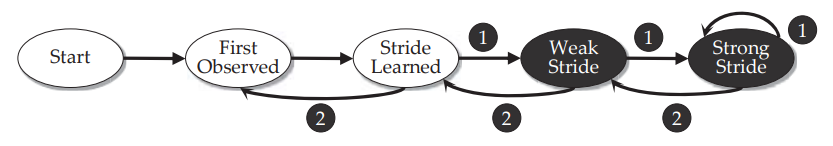
\includegraphics[scale=0.6]{stride-detector}
		\end{figure}
		
		This state machine keeps track of the stride length and position of previous accesses, inferring the stride length of the current access. The strong stride-weak stride states allow for short interruptions in otherwise consistent stride pattern. This may be helpful, for example, when accessing the rows of a two dimensional array. In this case, the access pattern may be unpredictable when switching between rows, but the overall stride pattern will remain the same. 
		
		\subsubsection{Data structure for non-strided accesses}
		
		Some memory access patterns are not strides. When this is the case, the SD$^3$ method calls these accesses ``points'', and puts them in a ``point table'', which is similar in structure to the pending and history tables in the naive method. These are kept separate from the strides, which are put in the ``stride table''. There is both a stride and a point table inside each history and each pending table. 
		
		\subsubsection{Data structure for strided accesses}
		
		Operations on non-strided accesses are efficient because the memory location of an access can be looked up quickly using hash tables. However, strides can conflict and be merged even when they don't start or end on the same address, so different data structures are needed. One possible method would just use a list of strides, but the pairwise comparisons needed to do conflict-check would take quadratic time. The SD$^3$ paper suggests use of interval trees to quickly prune the search space to mitigate this quadratic complexity.
		
		An interval tree is an augmented binary search tree that allows searches for intervals, instead of single values. An interval tree can efficiently find all intervals stored inside it which overlap with another interval. 
		
		Take the tree in Figure \ref{fig:interval-tree}, which stores 5 intervals, including \texttt{[20,30)}, \texttt{[10,15)}, and \texttt{[0,1)}. 
		
		%(WIKIPEDIA: \url{https://en.wikipedia.org/wiki/File:Example_of_augmented_tree_with_low_value_as_the_key_and_maximum_high_as_extra_annotation.png})
		
		\begin{figure}[h]
			\caption{Interval Tree}
			\label{fig:interval-tree}
			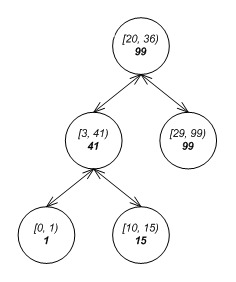
\includegraphics[scale=0.5]{interval-tree}
		\end{figure}
		
		This tree can be queried to find all intervals that overlap with another one, say \texttt{[40,50)} (this will return \texttt{[3,41)}, and \texttt{[29,99)}). Like an ordinary binary search tree, it is self-balancing and allows $O(\log(n))$ inserts and deletes. Finds are $O(m\log(n))$, where $m$ is the number of intervals it finds. 
		
		In the context of strides, each stride would simply be stored as an element in the tree keyed as an interval from first to last, inclusive. Then sets of strides will be looked up with efficiency relating to the total number of strides found, rather than the size of the set of strides. 
		
		\subsubsection{Merging strides}
		
		A simple way to MERGE two sets of strides is to join them together. However, this does not result in any compression. The online detection method generates strides for single accesses, which are immediately put in the pending table. So unless the adjoining strides in the history table are merged together with these strides during MERGE, the memory performance will not improve over the naive version. 
		
		Two strides are mergeable when they can be written as a single stride. For example \texttt{(first:1, last:10, interval:3)} and  \texttt{(first:13, last:22, interval:3)} can be merged, since the stride  \texttt{(first:1, last:22, interval:3)} covers the same elements as the two of them combined. On the other hand, \texttt{(first:2, last:8,} \linebreak\texttt{interval:2)} and \texttt{(first:13, last:22, interval:3)} cannot be merged since simply extending the bounds of the stride cannot include all of the elements of both strides.
		
		SD$^3$ uses the interval tree described above to find possible candidates for mergable strides, and then checks further. If strides for a particular instruction are consistently not found to be mergable, then no further attempts are made to merge them. 
		
		\subsubsection{Finding overlap between sets of strides}
		
		During CONFLICT-CHECK, there are 3 different types of possible access conflicts: point-point, point-stride, and stride-stride. Point-point conflicts are found exactly as in the naive version, with hash table lookups. Possible point-stride and stride-stride conflicts are found using interval trees. Checking point-stride conflicts efficiently is simple, but checking stride-stride conflicts in constant time is more complex. 
		
		SD$^3$ introduces a new algorithm called Dynamic-GCD which efficiently finds overlap between strides. 
		To understand how constant time stride overlap checking is possible, consider infinite length strides. Take two infinite length strides, with stride length $a$ and $b$. Take two points, one from each stride, and calculate the distance between them. Call this distance $c$. Then there is an integer $x$ and $y$ such that $ax + by = c$ iff the strides conflict. This condition is in turn equivalent to $c = 0 \mod (\gcd(a,b))$, where $\gcd(a,b)$ is the greatest common denominator of $a$ and $b$. This test can be done in constant time with the well known Euclidean algorithm for the GCD. Now, finite strides sometimes do not intersect when their infinite counterparts do, so the Dynamic-GCD algorithm gives a similar, but more complex test than the above that uses the Extended Euclidean algorithm to exactly compute intersection for finite strides. 
		
	\section{Bit compression}\label{s:bit-compress}
	
		A strided format is not the only method of compressing memory accesses. Memory accesses can also be compressed effectively using bit arrays. A bit array is simply an array of boolean variables which are stored inside individual bits, instead of in bytes, like ordinary C variables. 
		
		\subsection{Basis of bit compression}
		
		Stride compression is effective because many memory intensive procedures in real applications access memory in a strided fashion. Bit compression is effective because program memory is locally dense, meaning if memory is accessed in one location, nearby memory addresses are usually also valid program memory which will be accessed eventually. This local density property is virtually guaranteed by modern operating systems and hardware, and so it is not as dependent on the program's structure as stride compression. 
		
		\subsection{Implementation of a bit compressed integer set}
		\label{s:bit-set-comp-impl}
		
		A locally dense set implementation should use the advantages of dense and sparse set implementations. 
		A sparse set of integers is best implemented using a hash table. A completely dense set of integers is best implemented using a bit array. So a locally dense set should be implemented by a hash table where each entry is a bit array that represents a contiguous range of integers starting at a particular location. Figure \ref{fig:bit-local-density} shows the the three different types of sets storing the set $\{0, 3, 10\}$. 
		
		The items in the hash table in the locally dense set are key value pairs. The key in a key value pair is a unique identifier to a location in the table. The value is other information 
		
		\begin{figure}[H]
			\caption{Representations of the set $\{0, 3, 10\}$}
			\label{fig:bit-local-density}
			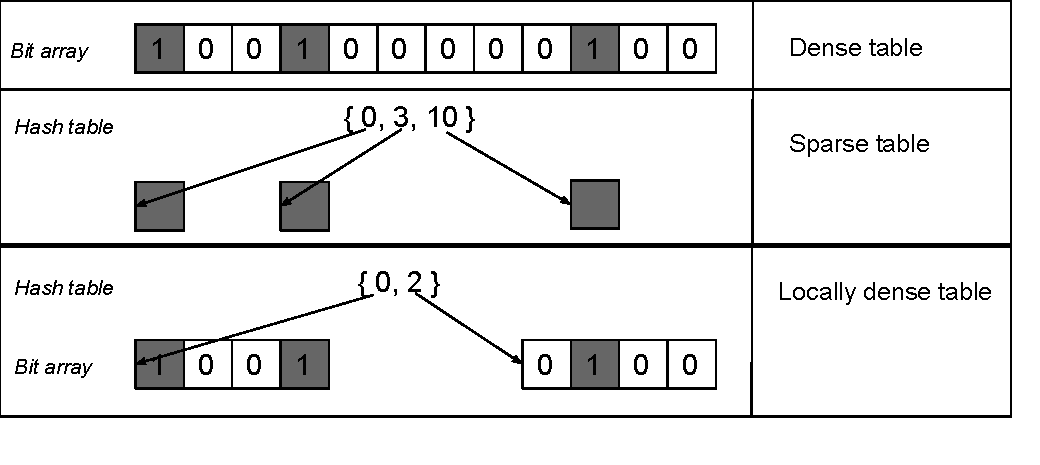
\includegraphics[scale=0.8]{BitSetComparison.pdf}
		\end{figure}
		
		
		
\chapter{Implementation}


	%There are several components that we implemented. 
	This chapter will first discuss workload characterization concepts, introducing the relevant hardware concepts, and then discussing our method of collecting specific characteristics in formats which can be matched with parallelism data. 
	
	To detect parallelism and also to compare the compression methods outlined in Section \ref{s:optimize-pairwise}, we implemented three different versions of the pairwise method: one based on stride compression, one based on bit compression, and one based on the naive implementation. This chapter will describe the stride compression and bit compression algorithms in detail. 
	

	\section{Introduction to workload characterization}
		\label{s:workload-characht}
	
		Workload characterization measures how applications use hardware features. %Workload characterization uses dynamic analysis to collect the runtime characteristics of a set of applications. %running on some set of hardware and of the software. 
		Hardware researchers are interested in the sorts of hardware characteristics that are important to application performance. They use workload characterization to understand how trade-offs in hardware design would affect various applications' performance. To accomplish this, they collect metrics on the applications they want to optimize. These metrics inform decisions about the of hardware trade-offs that hardware engineers are considering. 
		
		We are interested in a related question: What are the application characteristics that can help the programmer choose between different established hardware platforms? We use workload characterization to understand the platform independent characteristics of single threaded CPU programs that are indicators of performance for traditional multiprocessors and GPUs. 
		
		In this work, we examine a variety of applications that are best fit for CPUs and GPUs and collect platform independent metrics that help indicate which type of hardware that parts of the application are best fit for. %ay be important to distinguishing between
		%In thi gathered applications and platform independent metrics that indicate important differences between the different hardware platforms. 
		
		\subsection{Important hardware characteristics under consideration}
		
		%This thesis identifies several different hardware features as important, and attempts to capture in metrics. 
		
		In the following sections we explain some important hardware characteristics in traditional multiprocessors and GPUs and the metrics that measure some aspect of these characteristics. 
		
		\subsubsection{Scale of Parallelism}
		
		%GPUs will not be faster than CPUs unless there is a high degree of parallelism, and substantial work to be done.
		GPUs will not be able to execute procedures faster than CPUs unless that procedure has a high degree of parallelism. 
		GPUs have hundreds of small cores, where CPUs have at most two dozen or so larger cores. So CPUs are better at processing a small number of tasks; GPUs will not be effective unless the work can be split over hundreds of threads. To capture this, we suggest using the number of iterations in parallel loops.
		
		In addition, using a GPU has significant overhead, meaning it takes substantial time to run any computation on a GPU, no matter how trivial. This is because when a GPU is used, the CPU typically has to send data and code to the GPU, the GPU runs the computation, and then sends back the data. On a traditional multiprocessor, the overhead of using threads is much smaller. %This communication is slow compared to on-chip multiprocessing.
		
		Since each kernel call must do substantial work to be effective on a GPU, %, because the overhead of calling kernels is sometimes very high.  
		we suggest collecting the number of instructions each loop iteration contains to make sure there is substantial work to be done by the loop.
		% memory must be transfered back and forth between In addition, if the computation is extremely simple, say,  sometimes the cost of tran
		
		%GPUs are only useful when the algorithm can be divided into many threads, each of which has substantial content.
		
		%GPUs can run hundreds of threads have hundreds of are only useful when 
		
		
		\subsubsection{Parallelism Model}
		
		At a low level, GPUs execute threads in groups called warps. Warps have an SIMT (single instruction multiple thread) model of execution, meaning that each thread in the warp executes instructions simultaneously in lock-step. Due to this hardware design, when GPU threads in a warp execute different instructions due to a branch, they cannot do so simultaneously, so instead the different instructions are executed serially.\footnote{\cite{Fung:2007:DWF:1331699.1331735}} This sequential processing of branch paths creates a performance hazard called branch divergence. Handling branch divergence is time consuming on GPUs, so performance suffers significantly when branch paths differ within a warp.
		
		Meanwhile CPUs have a MIMD (multiple instruction multiple data) model, where each thread executes code independently. CPUs are also equipped with advanced branch prediction which often reduces the cost of branches to nearly zero. Consequently, parallel code which executes different branch segments may run better on CPUs. 
		
		To account for this performance difference, we collect a count of the number of conditional branches encountered, and the number of times the path of that branch changed. These branch changes capture the probability that different threads in a GPU warp will take different branch paths. 
		
		\subsubsection{Predictability of memory accesses}
		
		GPUs have global memory that is optimized for high bandwidth and high latency. Predictable accesses such as strided memory can be streamed from GPU memory to the cores efficiently, while unpredictable memory accesses stall the instruction pipeline because they take longer to access. 
		%[CITATION???] possibly file:///C:/Users/weepi/Documents/thesis/papers/CCWS.pdf 
		In contrast, CPUs have larger caches that accommodate data reuse, and so are much better at handling unpredictable memory if that memory fits inside the caches. % also benefit from predictable memory accesses, but to a lesser extent, since the memory structure is optimized towards lower latencies. 
		
		We chose to capture this performance difference by measuring the number and length of strided accesses. 
		We use the same stride detector code as in our pairwise method (see section \ref{sse:stride-descr}.2 for a design). 
		
		% Then, we simply count the number of accesses which are of certain stride lengths, including zero length strides, and those that cannot be detected as strides. 
		
		\subsubsection{Inter-thread vs Intra-thread memory sharing}
		
		CPU theads have much larger cache capacity than GPU threads, since there are simply many more GPU threads active at a given time.\footnote{\cite{Jia:6835938}} This means that GPU threads cannot rely on caches to exploit temporal or spacial locality to the same degree that CPU threads can. Instead, GPU caches effectively exploit cross-thread locality. 
		
		To capture this, we measure the amount of memory shared between loop iterations vs reaccessed within a single iteration.
		We construct maps of the memory footprint of the loop and each of its iterations. From these memory footprints, we calculate the number of unique memory bytes accessed in each iteration and each loop instance. %From that, the number of shared bytes between threads 
		
	\subsection{Loop-level Metrics}
		
		An important contribution of this thesis is creating tools which allow parallelizability information to be combined with other metrics in our workload characterization. 
		In particular, since we evaluate loop level parallelizability, we chose to collect all other metrics at the loop level. 
		
		We chose some metrics based on the main differences between CPUs and GPUs as described previously in this section, as well as some other metrics which are common in workload characterization. Table \ref{table:sum-data} summarizes these metrics. 
		
		\begin{table}[h]
			\caption{Summary of collected data}
			\label{table:sum-data}
		\begin{tabular}{ |p{6cm}|p{7cm}| }
			\hline
			Metric & Relevant hardware characteristic(s) \\
			\hline \hline
			Number of iterations & Scale of Parallelism \\
			\hline
			Instruction count of loop iterations  & Scale of Parallelism \\
			\hline
			Number of writes/reads & Traditional workload characterization \\
			\hline
			Bytes accessed per instance & Traditional workload characterization \\
			\hline
			Total memory footprint of loop & Memory sharing  \\
			\hline
			Shared memory footprint between loop iterations & Memory sharing \\
			\hline
			Strided accesses  & Memory access predictability \\
			\hline
			Number of branch changes & Parallelism type\\
			\hline
		\end{tabular}
		\end{table}
	



	\section{Metrics Collection}
	
		For a tool to detect loop level parallelism and collect loop level metrics, it first needs to understand where the loops are in the code. To do this, we run LoopProf (discussed in Section \ref{s:loopprof-detection}) on the application to collect information about which instructions loops start and end on. 
		
		To detect parallelism, we created a tool powered by Intel Pin\footnote{\cite{Luk:2005}} which uses the loop information generated by LoopProf. This tool calls methods from the parallelism detection algorithm when loops start and end, and when memory is accessed. When the program finishes, the parallelism detection algorithm outputs its results of how many loop iterations conflicted and which pairs of instructions those conflicts originated from. 
		
		To collect loop level metrics we created another analysis tool powered by Intel Pin\footnote{\cite{Luk:2005}} which uses the loop information generated by LoopProf. 
		Similarly to the pairwise method, this tool collects loop level information by keeping a stack of data about each current active loop, and when the loop terminates, it does two things. First, it accumulates the information about the current loop instance into a summary of all the instances in the static loop. Then it simply passes its information to the loop below it on the stack, which accumulates that information with its own information. 
		
		\subsection{Stack and register memory}
		\label{s:stack-reg-con}
		
		One problem with our approach to parallelism detection is that it has no way of detecting inductions. An example of an induction variable is the \texttt{i} in Code Example \ref{ce:induction}. According to the method of analysis demonstrated in Section \ref{s:nested-loop-demon}, the variable \texttt{i} carries a loop dependency because it is read in line 3 and then written in line 3. But this loop can be transformed into a parallel loop easily. This is a serious problem, since \texttt{i} is just a loop index that nearly every sequential loop has, including the ones that can be run in parallel. 
		
		Real world parallelism detectors use static analysis to detect these induction variables.\footnote{\cite{Kim:2010}} Static analysis is effective in this case because loop indices are almost always stored in a fixed location in the stack or in registers, so only fixed locations of memory need to be checked for the properties that induction variables have.
		
		Unfortunately, we did not have time to do any static analysis. To deal with this issue, our Pin tool which records accesses simply ignores all stack and registers access. While this means we do detect parallel loops, it also means that some problematic memory conflicts are not detected. 

\begin{codeexample}
	\caption{Loop Induction}
	\label{ce:induction}
\begin{lstlisting}
int i = 0;
while(i < 1000)){
	i = i + 1;
}
\end{lstlisting}
\end{codeexample}
		
		One example of a problematic dependency carried in registers is the \texttt{carry} bit in multiprecision addition.
		Say you have 2 numbers of arbitrary size, \texttt{A}, and \texttt{B}, and are putting the result in \texttt{R}. These are stored as arrays where \texttt{A[i]} is the \texttt{i}th 64 bit block of \texttt{A}. Then Code Example \ref{ce:multi-addition} shows an algorithm to compute addition. Note that the \texttt{carry} variable is a non-trivial dependence would could force this algorithm to be run sequentially. 

\begin{codeexample}
	\caption{Arbitrary-precision Addition}
	\label{ce:multi-addition}
\begin{lstlisting}
carry = 0
for(int i = 0; i < max_size(A,B); i++){
	R[i] = A[i] + B[i] + carry;
	if(addition_overflowed(A[i] + B[i] + carry)) {
		carry = 1
	}
	else{
		carry = 0
	}
}
...
\end{lstlisting}
\end{codeexample}	
	
		These register and stack dependencies seem to be rather rare in simple code, because finite quantities of memory rarely store crucial dependencies. But for more complex code, it seems more likely that such dependencies occur with some frequency. So when interpreting the results of this work, it is important to realize that our analysis assumes that stack and register variables do not cause problematic data conflicts. 
		
		
	\section{Workloads}
		\label{s:workloads}
		
		To distinguish between applications that are best run on CPUs or GPUs, we first needed a good sample of programs with different characteristics. Some of these should be geared towards CPUs, and others should be likely candidates for GPU acceleration. To get a wide variety of applications, we gathered applications from two different benchmarks: Rodinia and Parsec.
		
		\subsubsection{Rodinia}
		
		Rodina is a benchmark suite designed to compare CPU and GPU performance on different applications. The Rodinia applications are chosen to reflect the Berkley 7 dwarves of scientific computation.\footnote{\cite{Che:2010}} All of these applications are parallelizable to some degree, and most of them are effective on GPUs. 
		
		For each algorithm, Rodinia has a CPU implementation which is multi-threaded using OpenMP. Since our tool does not support multithreaded applications, we removed the OpenMP compilation flag, and removed calls to the OpenMP library such as \texttt{omp\_get\_thread\_num()} from the source code. 
		
		\subsubsection{Parsec}
		
		Parsec is a benchmark of multi-threaded applications designed for multiprocessors.\footnote{\cite{Bienia:2008}} It has a more diverse range of applications than Rodinia, including computer vision and textual analysis as well as traditional scientific computing applications.
		
		Parsec was more difficult to get running on our system. There were some applications which were incompatible with C++11, and did not compile, and many others which could not be altered to run single threaded without substantially changing the structure of the code, and so they could not be run on our analysis tools. We present results only for the applications that we could successfully compile and run on our tools. 
		

	
	\section{Stride Compression Implementation}
	
		The code that Kim et al. wrote to implement the SD$^3$ algorithm was not made publicly available, so it is closed source, and we cannot use it to detect parallelism. To achieve the goals of this thesis, we still needed to detect parallelism without running out of system memory, so we chose to implement the algorithm ourselves. As we had limited time to implement it, we decided to make changes to the algorithm for simplicity. In particular, we thought implementing interval trees ourselves would be error-prone, and we could not find an open source C++ implementation, so we chose to use other data structures. 
		In addition, the details of the Dynamic-GCD algorithm proved difficult to work out, so we used other techniques for finding stride conflicts.
		These were key features to ensure efficiency in the original SD$^3$ algorithm, so more changes had to be made to improve efficiency. In particular, a slow conflict-check method was used in our implementation, so optimizations were made that minimize the number of conflict-check operations that occur. 
		
		\subsection{Algorithm and data structure overview}
		
			
			First, a high level overview of the main data structures and objects will be introduced, and later the specific data structures and algorithms will be detailed. 
			
			At the highest level, a program has a single LoopStack, which contains a stack of LoopInstances. LoopInstances store all information about a particular active loop, including the pending and history tables.	Separate from the LoopStack, there is a StrideDetector for each instruction that accesses memory. 
			
			Recall from Algorithm \ref{basic-pariwise} that there are several main procedures in the pairwise method:
			
			\begin{enumerate}
				\item During a loop iteration, and when some memory is accessed, add the memory access and the instruction that accessed it to the pending table.
				\item After a loop iteration finishes,
				\begin{enumerate}
					\item Check for conflicts between accesses in the pending and history tables. This is referred to as Conflict-Check.
					\item Merge the pending table into history table.
				\end{enumerate}
				\item After an entire loop ends,
				\begin{enumerate}
					\item Merge all non-killed accesses in the history table into the pending table.
				\end{enumerate}
			\end{enumerate}
			
			Our stride compression implementation has three main data structures inside each pending or history table. The purpose of these data structures is outlined here, and the details will be explained later. 
			
			\begin{itemize}
				\item StrideTable: This table stores strided accesses and the corresponding addresses of the instructions from which the strided memory accesses originated. Strides can be added efficiently to this table.
				\item PointTable: This table stores non-strided accesses called points and the corresponding addresses of the instructions from which these memory accesses originate. 
				\item AddressSet: This structure is simply a set of memory addresses.
				This is in contrast to Point and Stride tables which also store the instruction addresses associated with each memory access. We found it necessary to store this separate table which stores strictly less information to enable one of our optimizations. %, without instructions. It has ordinary set operations, such as union, intersection, set subtraction, and inserting elements. It is used as an optimization only, as it stores strictly less information that the point and stride tables. 
			\end{itemize}
		
			These data structures store the content of the pending and history tables. Figure \ref{fig:loopinstance} shows how these tables fit inside the LoopInstance. Note that within a history or point table, there are two StrideTables, PointTables, and AddressSets, one table for reads, and one for writes.% are separate tables for each of but reads and writes are stored separately. See
			
			\begin{figure}[H]
				\caption{LoopInstance Layout}
				\label{fig:loopinstance}
				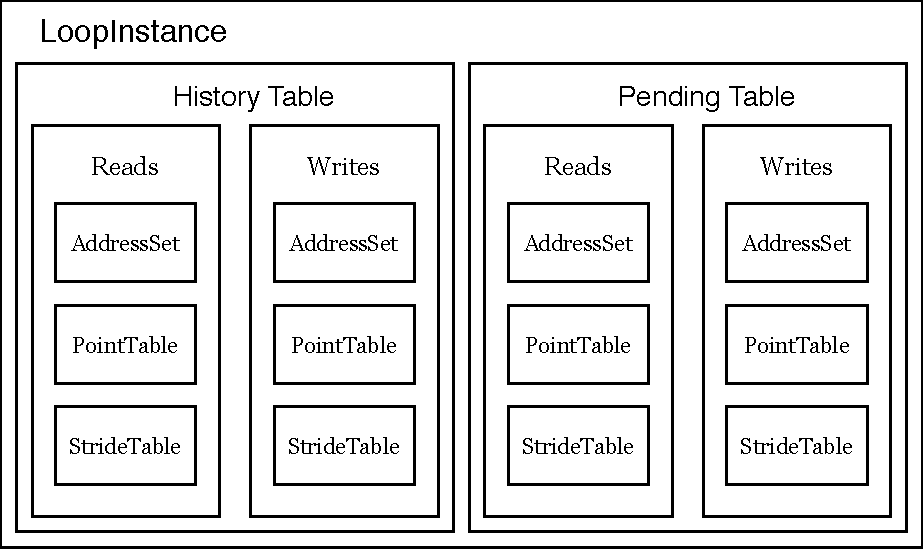
\includegraphics[scale=0.7]{loop-instance.pdf}
			\end{figure}
			
			
		\subsection{Adding accesses}\label{s:add-accesses}
		
		Algorithm \ref{new-memory-acc} provides a high level description of how new memory accesses are put in the pending table. Figure \ref{fig:add-access} shows the steps as a flow chart. The numbers in the figure correspond to the steps in the algorithm.% a lot of details out. These details will be explained here. 
		
		\begin{algorithm}
			\caption{New memory accesses}\label{new-memory-acc}
			When a memory location $m$ is accessed by instruction $i$, and LoopInstance $L$ is at the top of the loop stack,
			\begin{enumerate}
				\item If the memory location $m$ is killed according to the pending table's AddressSet, do nothing and skip the rest of the steps. 
				\item Add the bytes accessed by $m$ to the appropriate AddressSet.
				\item Find the loop-independent stride detector that corresponds to instruction $i$, and use it to calculate whether $m$ is a stride. It can be viewed as a stride, then look up the stride distance $d$ which was evaluated by the stride detector. 
				%\item Get the point table, stride table, and AddressSet of LoopInstance $L$ corresponding to the accessmode of $L$.
				\item If $m$ is a stride with stride distance $d$, then add it to the appropriate stride table.
				\item If $m$ is not a stride, add it to the appropriate point table. 
			\end{enumerate} 
		\end{algorithm}
	
		
		\begin{figure}
			\caption{Adding accesses}
			\label{fig:add-access}
			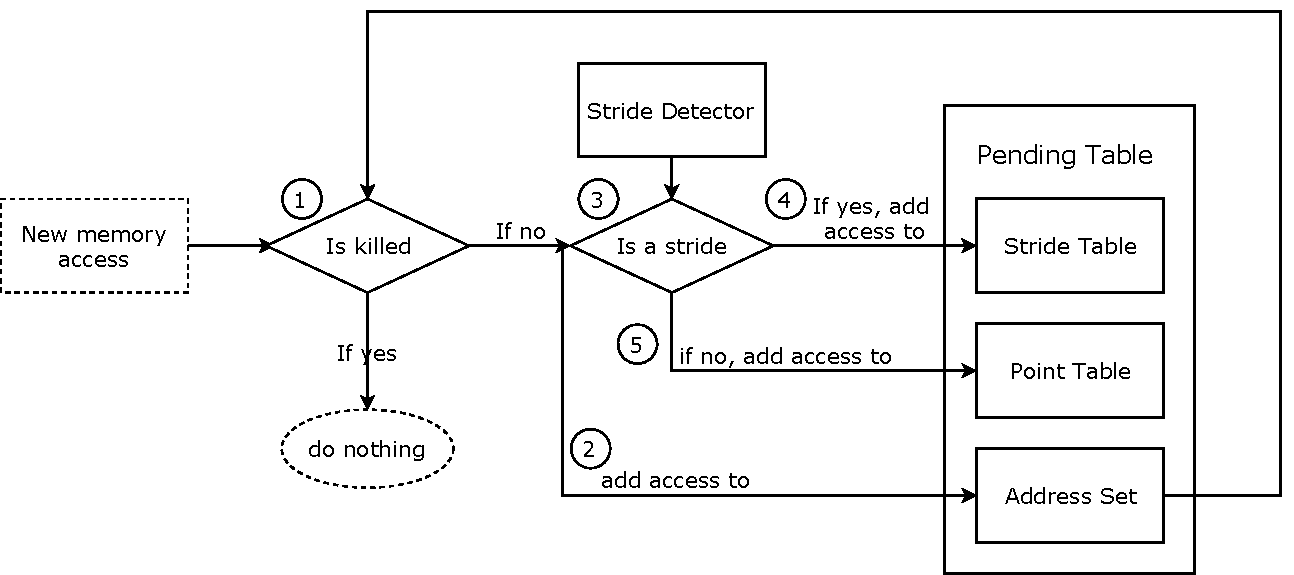
\includegraphics[scale=0.65]{add_access.pdf}
		\end{figure}
		
		
		\subsubsection{Stride Detection}
		
		The StrideDetector is implemented to match the original SD$^3$ design described in section \ref{sse:stride-descr} as closely as possible. The state machine matches Figure \ref{fig:stride-detector}.
		
		\subsubsection{Adding points to the PointTable}
		
			Points (non-strided accesses) are added to the PointTable during new memory accesses and merges of two tables. The PointTable is designed so that identical points are not duplicated in the table. 
			
			The PointTable is simply a set (no duplicates) of points matched by instruction address and memory address (see figure \ref{fig:point-table}). When being added to the PointTable, we check if the point already appears in the set.  If there is a matching element there already, nothing happens; otherwise, the point is added to the set. 
			%Recall that Points are specified by instruction address, memory address, and access mode (read or write). 
			%In Figure \ref{fig:point-table}, you can see that the a Point is stored for each instruction and memory address. 
			
			\begin{figure}[h]
				\caption{Point Table}
				\label{fig:point-table}
				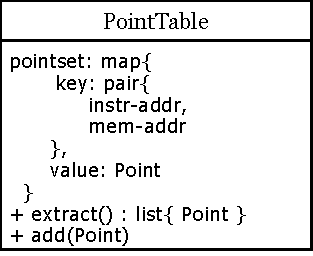
\includegraphics[scale=1.0]{point_data.pdf}
			\end{figure}
		
			
			%The data structures allow for a simple and efficient merge operation. The bit set is merged by an in-place union operation. For the point and stride tables, the operation simply calls \texttt{extract} to collect all the elements from the source table, and adds them one at a time to the destination table. 
			
			%The add operation is the only non-trivial operation. For points, it is straightforward: add the point if it is not yet there. This works because a point's location in the table uniquely specifies its value. 
			
			
		
		\subsubsection{Adding Strides to the StrideTable}
			
			Strides are also added to the StrideTable during new memory accesses and merges. 			
			When possible, strides need to be merged into existing strides in the table. This is critical for compression (see section \ref{sse:stride-descr}.5). The StrideTable is designed to make this process simple and efficient. 
			At a high level, the StrideTable is a set of ordered sets of strides. 
			Figure \ref{fig:stride-table} shows a precise outline of how the table is structured.  %The outer set ensures that a particular inner set contains only strides which are mergeable if they adjoin. The inner ordered set is used to check if the strides do adjoin, in which case, they are mergeable.
			
			\begin{figure}[h]
				\caption{Stride Table}
				\label{fig:stride-table}
				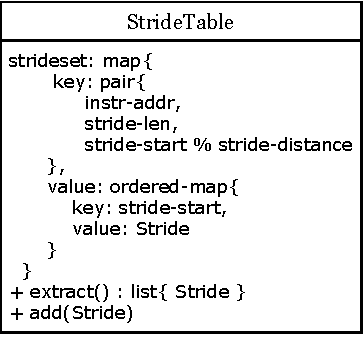
\includegraphics[scale=1.0]{stride_data.pdf}
			\end{figure}
			 
			
			When storing an element in the StrideTable, the outer set is matched on the instruction address, the stride distance, and the stride start modulo the stride distance. Strides which have these criteria in common are mergeable if they adjoin.  This is best explained with examples:
			
			\noindent
			\begin{tabular}{ |c||c|c|c|c| } 
				\hline
				Stride \# & Stride Distance & Stride start & Stride last & Merge issue with stride 1 \\ 
				\hline
				\hline
				1 & 2 & 4 & 8 & Mergeable \\ \hline
				2 & 2  & 0  & 2 & Mergeable \\ \hline
				3 & 3 & 4 & 13 & Stride distance \\ \hline
				4 & 2  & 5  & 9 & Stride offset \\ \hline
				5 & 2  & 14  & 20 & Not adjoined \\ 
				\hline
			\end{tabular}
		
			In the table above, stride 1 is only mergeable with itself and with stride 2. The other strides have the three types of issues which can prevent stride merging. Stride 1 is mergeable with stride 2 because the strides have the same stride distance, the same offset (they are both on the same numbers modulo 2), and they also adjoin (if stride 4 were one item longer, then its last element would be stride 1's first element). 
			Stride 3 has a different stride distance from the stride 1 so it is not mergeable with it. Stride 4 is not mergeable with stride 1 because it contain only addresses which are even, while stride 4 contains only odd addresses. This merging problem can be captured generally mathematically with the stride start modulo the stride distance.
			Finally, Stride 5 has the same stride distance and is on evens, but does not adjoin stride 1. The strides are not contiguous since 10 and 12 are not included in either, so stride 5 is not mergeable with stride 1.
			
			The type of non-mergeable accesses represented by strides 3 and 4 are separated out with the outer map of the StrideTable, which separates strides with different stride distances or stride starts into different ordered maps. 
			
			Now, the inner map needs to merge all adjoining strides, while not merging strides like stride 5. This problem is exactly the problem of merging of overlapping intervals, which is already well understood. But to be complete, a solution outline will be detailed here. % union of intervals, and is a much more well known pronl
			
			The inside map is ordered by the first element in the interval (which just happens to be a stride). Overlapping intervals are always merged, there will never be overlapping intervals in the map. This property will be used to guarantee efficiency.
			
			To see how this can be done, consider merging in stride 1 into the StrideTable when stride 2 and 5 were already added. 
			
			% below example, where there are three intervals in the table, and one intervals being added. The first intervals cannot be merged with the added intervals, and the other two can. 
			
			\newcommand{\bcl}{\cellcolor{black!50}}
			\begin{tabular}{ |l|l| } 
				\hline
				Current intervals & (0,2),(14,20) \\ 
				\hline
				Adding interval & (4,8) \\ 
				\hline
			\end{tabular}
			
			Since intervals in the table will never overlap, the interval directly below the added interval (the (0,2) interval) is the only possible interval that starts before it, and also could overlap. % In the example, this is (1,3) interval. 
			%
			The intervals above the added interval (in this case, (14,20)) can be efficiently checked because they are mergeable if their first element is less than the added interval's last element. %Then, it will merge every stride which starts after it starts, but ends before the added stride ends.
			
			%Two strides are possibly mergeable if they have the same instruction address, the same stride distance, the strides would be the same if they were infinite length. Referring back to Figure \ref{fig:stride-table}, these are exactly the strides which have the same value in the outer set, and so are placed in the same binary search tree. 
			
			%These criterion guarantee that any adjoining strides are mergable. The inner binary search tree is used to check if the strides do in fact adjoin. This is difficult because unlike an interval tree, only the start of the stride is ordered in the binary search tree.
			
		\subsection{Adding addresses to the AddressSet}\label{s:access-set}
			
			%The AddressSet stores a set of memory addresses. This is in contrast to Point and Stride tables, which also store the instruction associated with each memory access. We found it necessary to store this separate table which stores strictly less information as an optimization. It is critical in reducing the number of inefficient Find-Overlapping operations that are needed. It is also helpful for quickly checking killed memory locations. 
			
			%In particular, it allows us to improve the performance of certain operations which do not need instruction information. 
			
			%Since memory addresses are simply integers, we will discuss the implementation in generic terms of an integer set, rather than discussing memory addresses. To store this integer set efficiently, we use bit compression as discussed in Section \ref{s:bit-compress}.
			
			The AddressSet is implemented as a bit compressed set as described in Section \ref{s:bit-set-comp-impl}. That is, it is a table where each entry is a key value pair where the key is an integer which is equal to the $\lfloor \text{address}/\text{BlockSize} \rfloor$, and the value is a bit array of length BlockSize. Figure \ref{fig:bitset} shows a summary of this data structure. 
			
			
			\begin{figure}[h]
				\caption{AddressSet data structure}
				\label{fig:bitset}
				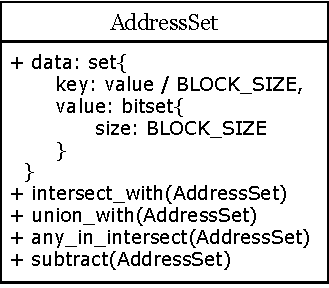
\includegraphics[scale=1.0]{bit_data.pdf}
			\end{figure}
		
			The table is implemented with a C++ \texttt{map}.
			The bit array is implemented with a C++ standard library's \texttt{bitset} which has fast intersection and union operations which are based on the C++ bitwise logical operators \texttt{\&} and \texttt{|}. Bit access and assignment are also simple to use, treated syntactically similar to array access, but are implemented as a mix of array accesses and bit twiddling. %, and are generally a little slower than accessing ordinary arrays. %, but are still fast enough to 
			
			New addresses can be added to the set with a single line of C++:
			%
\begin{verbatim}
bitset_table[memaddr / BlockSize][memaddr % BlockSize] = 1;
\end{verbatim}
			%
			This line depends on a quirk of the C++ \texttt{map} class: new entries are automatically created when accessed for the first time. 
			
			\subsubsection{Other operations of AddressSet}
			
			The AddressSet has other operations that are implemented. For example, during conflict checking, the intersection of the sets in the history and pending tables is taken, and during merging, the union of the sets is taken. 
			These operations follow a certain pattern. In-place set intersection is shown in Algorithm \ref{bitsetintersect} as a representative example of how these operations are evaluated. 
			%In line 2, the algorithm goes through the destionation of the sets item by item (in this case, the destination set). If the item is not in the other set, then the element is simply removed. If the item is in both sets, then it performs C++'s bitwise \texttt{\&} operator, which corresponds to set intersection on the bitsets. 
			The general pattern is to treat the map of bitsets like a sparse set, and if the two maps have a matching entry, then treat the bitset as a dense set. This method results in linear time operations with respect to the map in the for loop. 
			
			%So when a address is added to this set, it finds the block it is in by doing floor division by the BlockSize, and then setting the value of the address \% BlockSize bitset 
			
			%The Bit table stores a set of overall memory accesses, independently of the instruction it was accessed.
			
			%Points and strides store which instruction accessed them. But some operations do not need that information, they only need the overall memory accesses in the scope, independently of the instruction. We found it advantageous to store this information as well. It is implemented as a compressed bit set, described loosely in section 1.6. Here is a more precise description of the set's data structure:
			
			%Each of the operations are a combination of the obvious implementation for sparse sets, and the implementation for dense sets. Take in-place set intersection as a representative example. In a sparse set, in-place set intersection can be implemented by iterating through each element of the destination set, and deleting it if the element is not in the source set. In dense sets, the intersection is simply the boolean logical operation $x = x \land y$, applied to every bit. This can be implemented easily and quickly in C with the \texttt{\&} operator. Set intersection is implemented in the bit-set described above by treating the outer set as a sparse set, and the bit array as a dense set. See Algorithm \ref{bitsetintersect} for details. % going though each element of the source set, deleteing it is not in the destination set
			
			\begin{algorithm}
				\caption{BitSetIntersect}
				\label{bitsetintersect}
				\begin{algorithmic}[1]
					\Function{BitSetIntersection}{Dest,Src}
					\For{$\text{block},\text{bitset} \in \text{Dest}$}
					\If {$\text{blocknum} \in \text{Src}$}
					\State { bitset \texttt{\&=} Dest.get(blocknum)}
					\Else
					\State { Src.remove(blocknum)}
					\EndIf
					\EndFor
					
					\EndFunction
				\end{algorithmic}
			\end{algorithm}
		
		\subsection{Checking conflicts}
			
			In SD$^3$, there is a single procedure that evaluates memory conflicts using the point and stride tables. We broke this into two procedures for performance reasons.  The first procedure, IsParallel, is a fast operation that gives a binary answer: either the loop is parallel, or it is not. The second, slower operation, FindConflictingInstructions, finds the particular pairs of instructions which accessed the conflicting memory. Later, these instructions are reported to the user. FindConflictingInstructions is only run when IsParallel returns false, since there would never be conflicts in a parallel loop. Figure \ref{fig:conflict-check} shows the general outline of the relevant operations and data structures, which we describe below. 
			
			\begin{figure}
				\caption{Conflict-Check outline}
				\label{fig:conflict-check}
				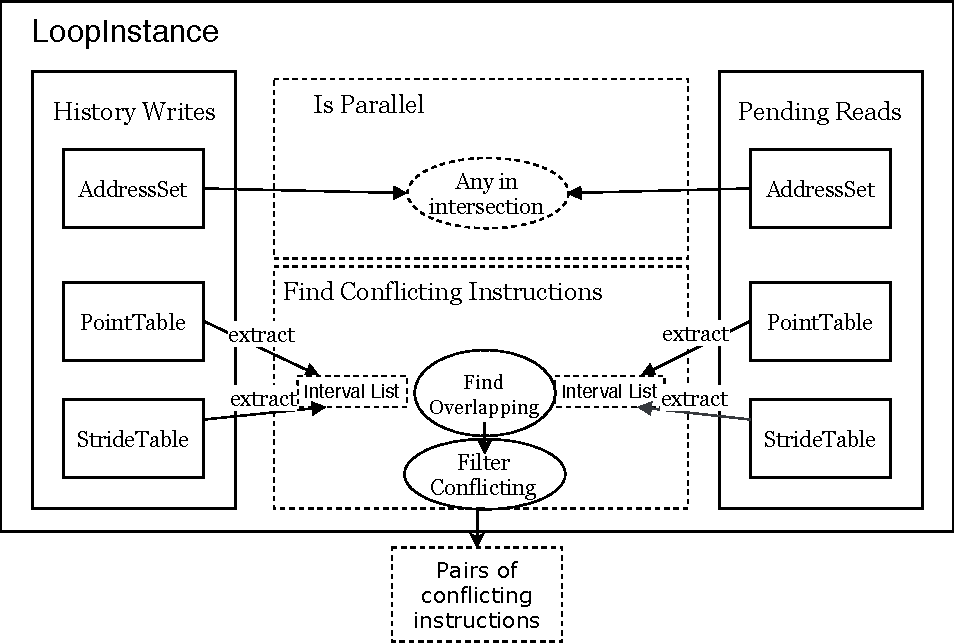
\includegraphics[scale=0.9]{conflict-diagram-output.pdf}
			\end{figure}
		
		\subsubsection{IsParallel}
		
			The AddressSet makes this operation simple and fast to compute. The intersection of the history write set and the pending read set is checked. The loop iteration is parallel if and only if that intersection is empty. If the intersection is not empty, this implies that a byte of memory has a read after write dependence which prevents the code from  being parallelized. 
			
		\subsubsection{FindConflictingInstructions}
		
			FindConflictingInstructions is broken into two steps. First, lists of all the strides and points in the stride and point tables are gathered. Then, these strides and points are treated as intervals, and the intervals that overlap are found in our FindOverlapping function. Finally, whether the strides and points actually overlap is calculated in our FilterConflicting function. 
			
		\subsubsection{Find Overlapping}
		
			FindOverlapping finds pairs of overlapping intervals. This is another well known interval problem. We use a sorted list technique. 
			The idea behind the algorithm is to sort the lists of intervals by their first element, and then going through all the intervals in one of the lists, and finding every element in the other list that overlaps with it. In order to do this efficiently, information about the second list is stored. % two lists while storing information about one of the lists. 
			Algorithm \ref{algo:findoverlapping} gives a precise description of this algorithm. %It takes in two lists, $A$, and $B$, and immediately sorts them. $A$ is simply traversed sequentially. $B$ is traversed as $A$ is traversed while keeping some properties true. These properties are as follows. The current interval of $B$ is the first interval that starts after the interval from $A$ starts (the \texttt{ib} variable in Algorithm \ref{algo:findoverlapping}). It also stores the intervals in $B$ that started before $A$ starts, and end before it ends (the \texttt{before\_last}).
			
		 	%From this, all the intervals from $B$ that overlap with the current \texttt{interval} from $A$ can be found quickly: The entire contents of \texttt{before\_last} overlaps with the \texttt{interval} from $A$. All intervals from $B$ which start before \texttt{interval} ends also overlap.
			
			%One of these lists will be gone through sequentially, call this list A.  go through one of the sorted lists, smallest to greatest, and moving through the the other list.  
			
			%a sliding window technique on sorted lists of intervals to compute a list of pairs of overlapping intervals. Call these lists A and B. The algorithm first sorts the two lists of intervals by their start. It considers each interval from A one at a time, call this interval $I$. It keeps a window of intervals of list B which overlap the start of $I$. Each time another interval from A is checked, the algorithm it drops the intervals which end before the new interval starts, and adds in all the intervals which start before the new interval starts, but end after it starts. Then it finds the intervals from B which start after $I$ starts, but before $I$ ends. Algorithm \ref{algo:findoverlapping} has psuedocode for this algorithm.
                    
\begin{algorithm}
    \caption{Find Overlapping}
    \label{algo:findoverlapping}
\begin{verbatim}
find_overlapping_intervals(A : interval list, B : interval list)
    sort A by first
    sort B by first
    overlap = Set()
    // before_last contains all interval from B that start before 
    // the current interval from A starts and end after the current
    // interval ends
    before_last = vector() 
    // ib is the first interval of B which starts after the interval
    // from A starts. 
    ib = 0
    for interval in A
        // removes elements from before_last efficiently
        new_before_last = vector()
        for item in before_last:
            if item.last >= interval.first:
                new_before_last.append(item)
        before_last = new_before_last
        
        // Find the ib that has the property for the current interval
        // while adding in new elements to before_last
        while B[ib].first() >= interval.first()
            if B[ib].last() >= interval.first()
                before_last.append(B[ib])
            increment ib

        // report overlaps for the intevals in before_last
        for bl in before_last
            overlap.add(bl,interval)

        // report overlaps for the intervals which start after
        // interval starts
        for ib2 = ib until B[ib2].first > interval.last
            overlap.add(B[ib2],interval)
            ib2 = ib2 + 1
\end{verbatim}
\end{algorithm}
		
		
		\subsubsection{Filter Conflicting}
		
			Recall that the SD$^3$ paper uses the efficient Dynamic-GCD algorithm to check if a pair of overlapping strides really do conflict. We found it difficult to work out the details of this algorithm, so we instead decided to use a different method. In particular, the vast majority of strided conflicts will be much easier to check for conflicts. We built our approach by making several observations about strides.
			
			\begin{enumerate}
				\item Many strides will be dense, meaning every byte in between the start and end of the interval will be accessed. Any overlapping strides are assumed to conflict if one of them is dense. This assumption is not always true and could result in false positives. 
				\item Many other possible conflicting strides will have the same stride distance. Then the strides conflict if the difference in the stride starts modulo the stride distance is zero. 
				\item Many strides will have long interval overlap compared to the stride distances. Formally this is calculated by $$\text{lcm}(\text{stride distance 1}, \text{stride distance 2}) < \text{interval operlap}$$ In this case, the ordinary GCD test described in Section \ref{sse:stride-descr} gives the correct answer.
			\end{enumerate}
			Our method verifies if an observation holds for a particular case. For example, in the first case, it checks if one of the two strides is dense. Then it uses the properties of the case to check if the strides really do conflict. For example, in the third case, by performing the GCD test to check if the strides conflict. 
			%Our method simply checks if these cases apply, and if so, calculates the answer.
			If none of the properties are found to hold for a given pair of strides, then the two strides are checked for conflicts with a slow algorithm which compares the strides element by element.
			 
			%In particular, it is important to note that having constant time comparison is not needed for algorithmic efficiency of the method. After all, each element of the stride is added one at a time, and it is only compari
			
			
		
		\subsubsection{Truncation of FindConflictingInstructions}
			
			Whether the loop has conflicts or not, we do not want to run FindConflictingInstructions for every loop iteration or else the algorithm would run in quadratic time with respect to the number of loop iterations, which would be untenable. We reduce the number of times we run FindConflictingInstructions to a constant number per loop instance by making two observations: 
			
			\begin{enumerate}
				\item If the loop iteration does not have any conflicts (discovered by running IsParallel), then we know that no instructions have conflicts, and we have no reason to run FindConflictingInstructions. 
				\item If the loop does have conflicts, then the same conflicts most likely occur in many other loop iterations. So, after we have found the locations of conflicts in some constant number of loop iterations, we simply do not check later iterations. The information reported may be incomplete, but some conflicts will always be reported.% We accept the imperfection of reporting 
			\end{enumerate}

			

			%The conflicting instructions are simply guides to the programmer. As such they do not have to be 100\% accurate. In particular, if there are some instruction conflicts which are reported, and others which are not, this is not a serious problem. So this information can be truncated.  
			
			Combined, these two truncation techniques mean that we have reasonably accurate reporting while only running FindConflictingInstructions a constant number of times for a particular loop instance.
			%more than a constant number of times in a loop 
			
			
	\subsection{Loop termination}
		
			When a loop terminates and it is not the outermost active loop, then it must be merged into its parent loop. Every Point and Stride is extracted from the outer loop's history table, and unless the point or stride has been killed, it is added to the inner loop's pending table using the add method described in Section \ref{s:add-accesses}. 
		
		\subsubsection{Killing points and strides}
		
			Recall that when a history table is merged into the outer loop's pending table, killed addresses must not be added to the pending table. 
			The SD$^3$ algorithm removes killed points and strides by a similar algorithm to their conflict-check method. We used AddressSets to do this instead. Given a particular point or stride, we simply use the AddressSet to check if the bytes that point or stride describe have been marked as killed. Strides and points are only removed if every byte they reference is killed. This could result in false positives when identifying conflicts. But we do not believe that this will be a common occurrence. %but it seems unlikely that partially killed points and strides are an important case. 
%			
%			AddressSets are first killed with set subtraction, and then unioned into the appropriate set. 
%			Stride and Point tables are merged by simply extracting every Point or Stride from the source table, and adding them one at a time into the destination table using the add method . 
%			
		
					
		\section{Bit Compression Implementation}
			
			Stride compression introduces all sorts of complexity, creates performance issues, and does not guarantee good compression on all workloads. Bit compression (introduced in Section \ref{s:bit-compress}) has the potential to be the basis of a much simpler, faster compression system. % with less reliance on program specific characteristics. 
			
			%This approach may not have been suitable for Kim et. al.
			%Unlike stride compression, it cannot even approximate
			
			\subsection{Main ideas}
			
			For our implementation, we combine the naive method's approach of listing instructions for each memory address, and bit compression's approach of breaking up the address space into contiguous blocks which are stored as bit arrays. This approach will allow us to keep track of instruction information while compressing memory addresses in bit arrays. 
			The interactions of these ideas are explained below.
			%Similarly to the naive method, accesses are grouped by their memory address, and instruction information is linked to. 
			
			Figure \ref{fig:naive-table} shows how the naive implementation stores the accesses listed in Table \ref{t:examp-acc}. The accessed memory addresses all store a list of instructions that accessed that address. For example, memory address 3 stores the list that just contains instruction 15. 
			
			\begin{table}[H]
				\caption{Example accesses}
				\label{t:examp-acc}
				\begin{tabular}{ |c|c| }
					\hline
					Instruction & MemAddress \\ \hline
					21 & 0 \\ \hline
					15 & 0 \\ \hline
					15 & 3 \\ \hline
					3 & 10 \\ \hline
				\end{tabular}
			\end{table}
			
			
			
			Figure \ref{fig:bit-comp-idea} shows how the bit compression implementation stores this same set of accesses with a BlockSize of 4. 
			Similar to  the bit compressed set described in Section \ref{s:access-set},\footnote{Note that the exact memory addresses accessed are identical to the example in Figure \ref{fig:bit-local-density}, so that figure can be used for additional context into this implementation.} the table splits the address space into fixed width blocks. Each block stores two things. Most importantly, it stores a map of instructions to the addresses in the block which that instruction accessed (second row of the BlockInfo). In order to speed up conflict-check, it also stores a bitset of overall accesses (first row of the BlockInfo). 
			
			This main data structure is used in the pending and history tables. Again, there are two of these data structures in each pending and history table, one for reads and one for writes. 
			
			\begin{figure}[h]
				\caption{Naive implementation table}
				\label{fig:naive-table}
				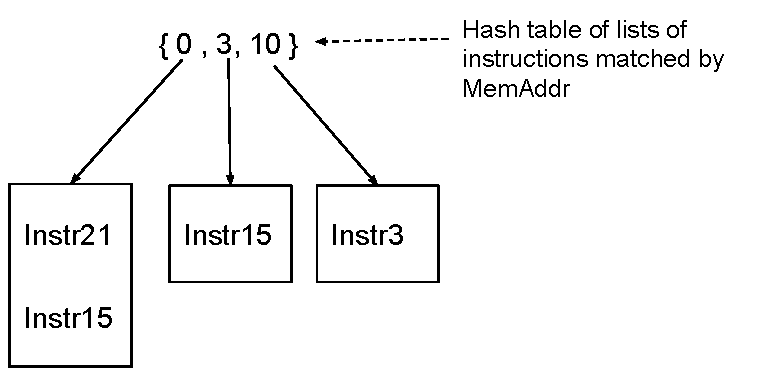
\includegraphics[scale=0.85]{BlockSetnaive_structure.pdf}
			\end{figure}
		
			\begin{figure}[h]
				\caption{Bit compressed table}
				\label{fig:bit-comp-idea}
				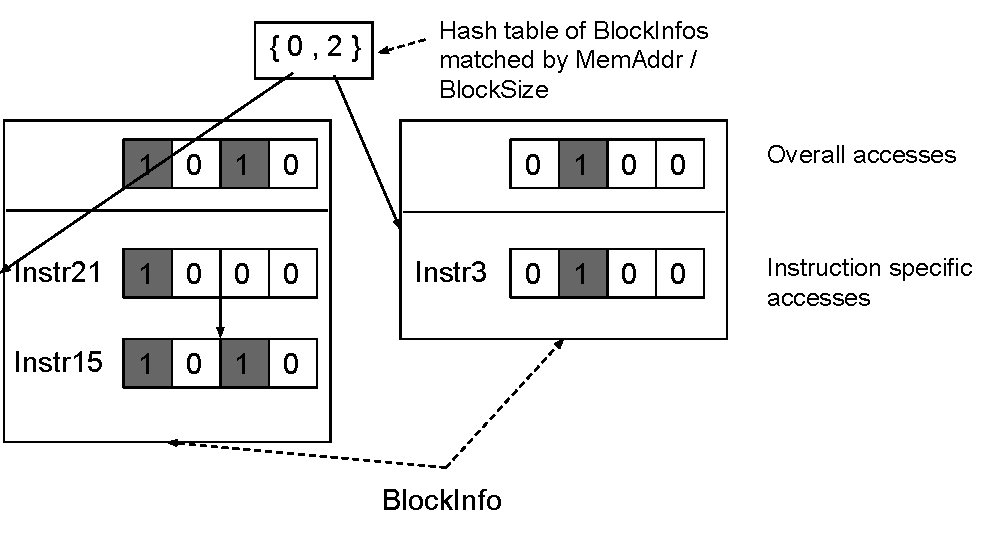
\includegraphics[scale=0.85]{BlockSet_accesses.pdf}
			\end{figure}
		
			\subsubsection{Implementation details of data structures}
			
			All key value maps in our bit compressed table are implemented with the C++ standard library \texttt{map}. Under the covers, this is implemented as a binary search tree, but we only use functionality that hash tables also have. 
			
			To implement the bit array, we use the C++ standard library \texttt{bitset}, which allows for simple bit access and assignment and also union and intersection operations. Under the covers, this is just an array of integers. The C++ \texttt{bitset}'s union, intersection, and set subtraction operations are extremely fast, because they are implemented with C++'s logical bitwise operations \texttt{|}, \texttt{\&}, and \texttt{\~}. These operations process all the bits in a single integer in parallel. 
			
			The address space is divided into blocks of 256 bytes, resulting in a 256 length bitset, which takes up 32 bytes of memory. This number was chosen because in the best case this allows for over 100 times the memory efficiency of the naive method, and in the worst case, it is only around 5 times worse than the naive method, since it only stores one blockset per instruction, and an instruction takes 8 bytes to store. 
			
			\subsection{Adding new memory}
			
			When a byte of memory is accessed by an instruction, then
			
			\begin{enumerate}
				\item If the byte is killed (meaning it appears in the write table, but not the read table), then do nothing, and exit.  
				\item If there is no BlockInfo element that covers the address in the pending table, then add an empty one. 
				\item Add the byte accessed to the overall accesses bitset inside its BlockInfo.
				\item If the instruction is not in the BlockInfo, add it.
				\item Add the byte accessed to the bitset associated with the instruction address.
			\end{enumerate}
			
			If multiple bytes are accessed by the same access, then this process is just repeated for each byte. 
			
			% the access is added to the BlockInfo, (the BlockInfo is put in the table if there is none there). 
			%is put in the accessed block of memory is first accessed,
			
			\subsection{Conflict-check}
			
			When the pending table is merged into the history table, pairs of conflicting instructions need to be found. 
			
			Note that an access can only conflict with other accesses that have the same block identifier, MemAddress/BlockSize. If a pending table has a BlockInfo specified by a certain MemAddress/BlockSize, and the history table does not, then none of the accesses in that BlockInfo element in the pending table conflict with any elements in the history table. 
			
			The non-trivial important case is when a BlockInfo element is both in the pending and history tables. 
			In the worst case, this is determined by comparing each pair of instructions in the respective BlockInfo elements, and checking if the intersection of their respective bitsets is empty. The overall access bitset is used to prune this computation, because if a bitset for an instruction does not conflict with the overall bitset in the other BlockInfo, then it also does not conflict with any of the instructions in that other BlockInfo. If the intersection is not empty, however, then a conflict exists between that instruction and at least one of the instructions in the other BlockInfo. Then the exact instruction(s) that conflict are found with exhaustive search.  %, giving the resulting algorithm.
			
%			\begin{enumerate}
%				\item Find the blocks in the read table of the pending table which overlap with blocks from the write table of the history table. 
%				\item If the intersection of the "union" property of the BlockInfo is empty, then the blocks do not conflict.
%				\item Otherwise, check each pair of instruction BlockSets in the BlockInfo to see which instructions do conflict. 
%			\end{enumerate}
			
			\subsection{Merge}
			
			Merging tables is as simple as merging the sets of instructions in the matching BlockInfo elements, and computing the union of the bitsets associated with a particular instruction in a BlockInfo. The union of the overall access bitset is also calculated. 
			
			\subsection{Killing accesses}
			
			Recall that the accesses which are written but not read in the pending table are killed, and no further access should be added.
			
			%So when adding new accesses, new accessed bytes are intersected
			
			So when merging the history table into the pending table, the bitset in the pending table which is the intersection of the write bitset and the negation of the read bitset is computed, and all instruction and overall bitsets in the BlockInfo at that location in the pending table are computed. 
			
\chapter{Results}
	
		\section{Intro}
	
		Having created the tools described in Chapter 2, we now evaluate the effectiveness of these tools when run on a set of applications. First we evaluate the memory consumption of the stride and bit compression implementations. Then, we examine how important the parallel loops are to the applications' performance. We select the parallel loops that are found to be important, and examine some characteristics of these loops including the degree of parallelism, the variance of the length of the loop iterations, and the scale of the loop. Finally, we examine the workload characterization metrics in important parallel loops. 
		
		%We also evaluate the degree and type of parallelism the tools find in the applications. We then focus attention on the most important parallel loops, and examine other characteristics of these loops found by the tool, including 
	
		%We have three main results: the , the potential usefulness of the parallelism detector for the programmer and for analysis, and the potential for matching parallelism with other metrics.
	
		\subsection{Running applications}
		
		All the results were obtained by running a set of applications selected from the Rodinia and Parsec benchmark suites introduced in Section \ref{s:workloads}.
		Table \ref{all-applications-table} lists all the applications we examined, the benchmark suites the applications came from, and the command line arguments used during our analysis. 
		
		Note that when the command line argument is a filename, it does not include the full path to the data file. The data files that are used are all ones that were included in the original benchmark suite; no new files were created. 
		
		
		\begin{table}
			\caption{Benchmark application and their inputs}
			\label{all-applications-table}
			\scriptsize
			\begin{tabular}{ |l|l|l| }
				\hline
				Application          & Suite   & Command line arguments  \\ \hline
				\hline
				B+tree & Rodinia  &  \texttt{b+tree.out core 2 file mil.txt command command.txt}  \\ \hline
				Back Propagation & Rodinia  &  \texttt{backprop 655360} \\ \hline
				Breadth First Search & Rodinia  &  \texttt{bfs 4 graph1MW\_6.txt}  \\ \hline
				%CFD & Rodinia  &    \\ \hline
				Heartwall & Rodinia  & \texttt{heartwall test.avi 5 4} \\ \hline
				Hotspot & Rodinia  &   \texttt{hotspot 1024 1024 2 4 temp\_1024 power\_1024 output.out} \\ \hline
				Hotspot3d & Rodinia  & \texttt{3D 512 8 100 power\_512x8 temp\_512x8 output.out}   \\ \hline
				kmeans & Rodinia  &    \texttt{kmeans -i kdd\_cup} \\ \hline
				lavaMD & Rodinia  &  \texttt{lavaMD -cores 4 -boxes1d 10}   \\ \hline
				%leukocyte & Rodinia  &     \\ \hline
				LU Decomposition & Rodinia    &  \texttt{lud\_omp -s 2000} \\ \hline
				Myocite & Rodinia  &  \texttt{myocyte.out 100 1 0 4}  \\ \hline
				Nearest Neighbor & Rodinia  &  \texttt{nn ./nn/filelist\_4 5 30 90}   \\ \hline
				Needleman-Wunsch & Rodinia  & \texttt{needle 2048 10 2}    \\ \hline
				ParticleFilter & Rodinia  &    \texttt{particle\_filter -x 128 -y 128 -z 10 -np 10000} \\ \hline
				PathFinder & Rodinia  &  \texttt{pathfinder 100000 100}   \\ \hline
				SRAD & Rodinia  &  \texttt{srad 2048 2048 0 127 0 127 2 0.5 2}   \\ \hline
				StreamCluster & Rodinia  &    \texttt{sc\_omp 10 20 256 4096 4096 1000 none output.txt 4} \\ \hline
				Black Scholes & Parsec  &  \texttt{blackscholes 1 in\_64K.txt prices.txt} \\ \hline
				Canneal & Parsec  &  \texttt{canneal 1 15000 2000 400000.nets 128} \\ \hline
				Facesim & Parsec  &  \texttt{facesim -timing -threads 1} \\ \hline
				Fluidanimate & Parsec  &  \texttt{fluidanimate 1 5 in\_300K.fluid out.fluid} \\ \hline
				Streamcluster & Parsec  &  \texttt{streamcluster 10 20 128 16384 16384 1000 none output.txt 1} \\ \hline
				Swaptions & Parsec  &  \texttt{swaptions -ns 64 -sm 40000 -nt 1} \\ \hline
			\end{tabular}
		\end{table}
		
	\section{Memory improvement of compression}
		
		Recall that the effect of stride compression on memory demands, and to a lesser extent bit compression, are contingent on program characteristics. To make sure that the compression methods we implemented are effective and to see how the two compression methods compare, we measured the memory consumption of these different approaches on the applications. 
		
		\subsubsection{Memory evaluation setup}
		
		The maximum memory consumption used by our tool while running an application was measured by querying the Unix \texttt{ps} utility approximately every 20ms over the entire run of our tool. The maximum of all such queries is reported as the maximum memory consumed. As such, the resulting memory consumption is only an approximation. In particular, if the program allocated memory and immediately freed the memory before \texttt{ps} was queried again, that additional memory would not be measured. We do not believe that this measurement issue will cause serious error in measuring our tool's memory consumption because the tool runs slowly and consumes large quantities of memory throughout the run. %However, that measurement error would only have a significant impact on programs with small memory consumption that run quickly,%, which certainly do not describe the pairwise method implementations.
		
		\subsubsection{Inadvisablilty of the naive method}
		
		
		\begin{figure}
			\caption{Memory consumption of parallelism detection on applications}
			\label{fig:mem-comp-plot}
			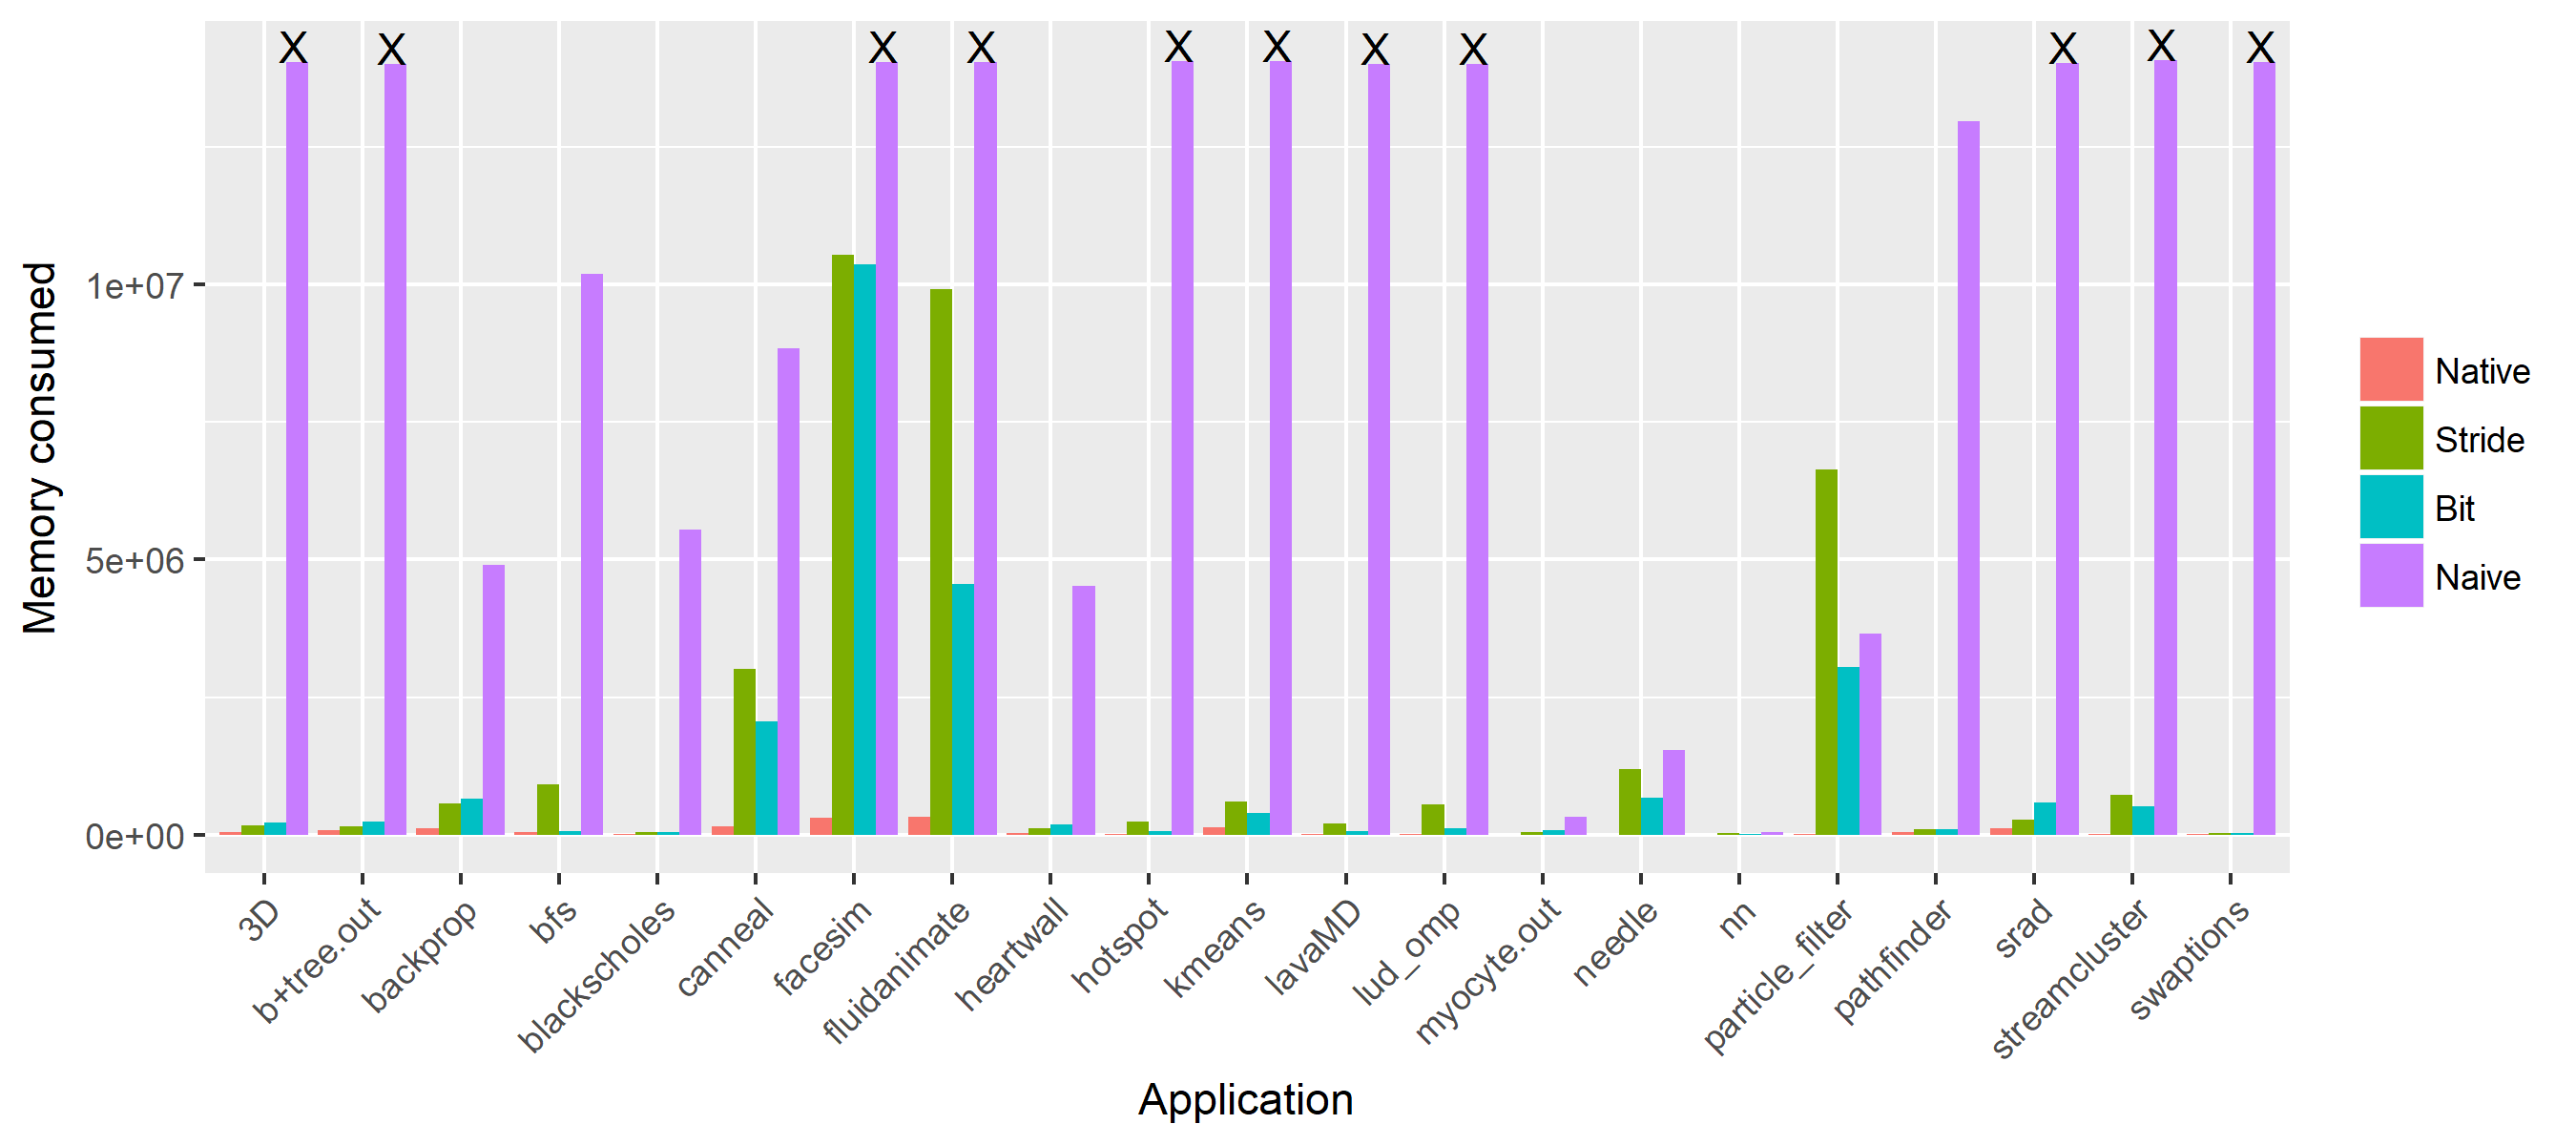
\includegraphics[scale=0.65]{plots/overall_plot.png}
		\end{figure}
		
		The naive method implementation often took up more memory than an ordinary desktop would have. The full results are plotted in Figure \ref{fig:mem-comp-plot}. Our system had 16GB of memory, and so the process was terminated after the program used over 14GB (on the plot, this is marked by an X). The naive method used more than 14GB of memory on 11 of the 21 applications, while neither the stride nor the bit compression methods used that much on any of the applications. This result confirms Kim et. al.'s observations that the naive method is not useful for important practical purposes, and that stride compression does help solve the problem.\footnote{\cite{Kim:2010}}
		
		%Next, note the huge variation in the absolute and relative overhead of all three implementations of the pairwise method. Sometimes the 
		
		%One question to ask is whether the stride method, with its additional complexity, but better theoretical compression, is better than the simpler and faster bit compression. 
		
		\subsubsection{Bit compression vs. Stride Compression}
		
		We now consider the respective memory overhead of stride compression\footnote{As a caveat, note that this stride compression implementation is not completely comparable to SD$^3$, since we added an AddressSet, which SD$^3$ does not store.} and bit compression. 
		Recall that in theory, stride compression can also do much better than bit compression. In the best case, stride compression can make profiling memory consumption independent of input size, as the entire working memory can be compressed into a single stride. Of course, this ideal scenario is highly unlikely in real programs, and in the worst case, little memory is accessed in a strided manner, and stride compression does no better than the naive version. Bit compression claims to be less dependent on program characteristics, as it stores blocks of contiguous accesses, but it can also do as poorly as the naive method in cases where each instruction only accesses a single piece of memory in each block. Determining which method is better needs to be measured on real applications. 
		
		Overall, the performance of the methods depends on the applications. As seen in Figure \ref{fig:mem-comp-plot}, bit compression sometimes performs better and sometimes worse than stride compression. For example, stride compression gets better results on \texttt{srad}, \texttt{heartwall}, and \texttt{backprop}, while bit compression does better on \texttt{bfs} and \texttt{fluidanimate}. But when bit compression performs better, it sometimes performs much better, while stride compression only does better by a little. For example, \texttt{srad} is the application where stride compression beats bit compression by the greatest margin, using only 47\% of the memory of bit compression. Meanwhile, for \texttt{bfs}, bit compression uses only 6.2\% of the memory of stride compression, a huge improvement.


%		To see why bit compression can do so much better than stride compression, consider the case of bfs. The runtime of bfs is dominated by processing the text input, which is a list of integer pairs that represent graph edges. For example, take the following:
%		
%		\begin{verbatim}
%		2541 3
%		3290 5
%		1114 6
%		3576 4
%		3647 4
%		\end{verbatim}
%		
%		%Text processing is not particularly stride friendly, since different instructions handle different parts of the text. 
%		This text will not be processed with highly strided acceses.
%		Assuming an ordinary implementation of text processing, the method to process the integer \texttt{2541} will exit when the space is hit, and then will start again when processing the integer \texttt{3}. But these will be stored as two short strides, not one, since the space in between the intergers is skipped. Bit compression stores whole blocks of memory, so the two sequences of accesses will most likely be put in the same block, and also the accesses created by processing the next few lines. %The actual implementation uses repeated calls to fread, but presumably under the covers something like this is going on.

		
		One explanation for why stride compression performs poorly while running \texttt{bfs} is because the main process of \texttt{bfs} is not stride friendly. In the \texttt{bfs} (breadth first search) code, the graph is implemented as an adjacency list. 
		%The inner loop of bfs traverses the edge list of a node, and touches another array based on the location specified by the edge. 
		Code example \ref{code:bfs} is the inner loop of \texttt{bfs} copied from the source code. The \texttt{h\_graph\_edges} array stores the edge list, and the value it stores is used as an index into the \texttt{h\_graph\_visited} array. Since the locations at which the memory is accessed is dependent on the values in the input, the accesses to the elements of \texttt{h\_graph\_visited} will not necessarily be strided, that is, separated from one another by a fixed distance. 
		
		These non-strided accesses will then be stored as points, consuming as much memory as accesses in the naive method. Since these accesses are a significant part of overall accesses in \texttt{bfs}, memory performance as a whole will suffer. 
		
\begin{codeexample}
	\caption{Breadth first search inner loop}
	\label{code:bfs}
		\begin{verbatim}
for(int i=h_graph_nodes[tid].starting; 
     i<(h_graph_nodes[tid].no_of_edges + h_graph_nodes[tid].starting); 
     i++) {
    int id = h_graph_edges[i];
    if(!h_graph_visited[id]) {
        h_cost[id]=h_cost[tid]+1;
        h_updating_graph_mask[id]=true;
    }
}
		\end{verbatim}
	\end{codeexample}
		
		Another surprising result is that the naive method uses comparable memory to the compressed methods on several applications, most notably \texttt{particle\_filter} and \texttt{needle}. This suggests that there are some applications which neither compression method works effectively on. 
		
		%This give evidence for the possibility that bit compression gives more reliable compression ratios than stride compression. To 
		
		%that the bit compression method is often 
		
		\subsection{Future work}
		
		Applications are continuing to become more and more memory intensive, so we will continue to need better memory compression methods to support that growth. We were considering using the SPEC 2017 applications for this thesis, but found that some of the applications on ``train'' inputs were consuming too much memory for our analysis. When running the ``intspeed'' benchmark (a subsection of the SPEC 2017 benchmark), the deepsjeng\_s application natively used almost 7GB of memory. When running the fpspeed benchmark, the lbs\_s application used 3.1GB of memory.  
		Assume that these applications have similar compression ratios to \texttt{facesim}, which consumed 310MB natively, and the tools consumed around 10GB of the memory when profiling it. Then both of these applications could have an overhead of over 100GB, far more than ordinary systems have. 

		%These memory numbers far exceed that of the SPEC 2006 memory consumption on train inputs. 
		
		One possibility to improve compression ratios is to combine the stride and bit compression. This can be done by implementing the point table using bit compression, and possibly by putting small strides in the point table when they cannot be merged in with other strides. 
		
	
	\section{Identifying important parallelism}\label{s:important-paralleism}
		
		One of the goals of this thesis is to use parallelism detection to aid further analysis, for example estimating the effectiveness of GPU acceleration. 
		This section evaluates whether the parallelism tool we built can be used for this purpose. In particular, we confirm that the tool does detect loops which could possibly be accelerated by parallel hardware, including massively parallel hardware like GPUs, for meaningful performance improvements. 
		
		\subsubsection{Caveat for the correctness of results}
		
		As discussed in Section \ref{s:stack-reg-con}, the parallelism detector does not detect dependencies carried through stack and register variables. This implied that it may not give correct results on certain algorithms where dependencies are carried by local variables. While we believe that this is uncommon, this remains an unverified assumption, so all the results in this section should be evaluated in the context of that assumption.
		
		\subsubsection{Significance of loops}
		
		Most loops consume a tiny faction of the applications' running times. Programmers usually want to optimize entire applications; individual loops are only optimized when significant portions of the application's running time is spent in the loop. Since the performance of these loops are unimportant to the programmer, they are not worth investigating, and should be eliminated from further analysis.  
		%We found that certain loops, some parallelizable and some not, have outsized importance to program runtime. 
		Figure \ref{fig:size-iteration-plots} shows the percentage of running time spent in the loops (estimated by machine instructions executed), how many iterations these loops have, and whether the loops were found to not have data conflicts (which means they are parallelizable). This plot includes all loops from all applications. 
		%In the figure, loops which are parallel, and have a large number of iterations (blue dots, upper left) have a good chance of being usefully parallelized on GPUs. 
		%Loops which are not found to be parallel, but do have a large number of iterations, and are important (red dots, upper left) can be reported to the programmer as worthy of further investigation. Perhaps they can be parallelized with a reduction or with some data synchronization. 
		
		%In this plot, as with the all of our analysis, running time is estimated with number of machine instructions executed. 
		%We use the proportion of instructions evaluated in the loop to estimate how much time is spent in a loop. % we estimate the percentage of time spent in the loop. This is estimated b calculate the %evaluate how important  is a metric for loop importance relative \
		%This metric is placed as a function of loop iterations is displayed on Figure . The higher the loop is on the graph, the more important it in the application performance.
		
		\begin{figure}
			\caption{Loop importance and parallelizability}
			\label{fig:size-iteration-plots}
			
			\begin{minipage}{0.73\textwidth} % choose width suitably
				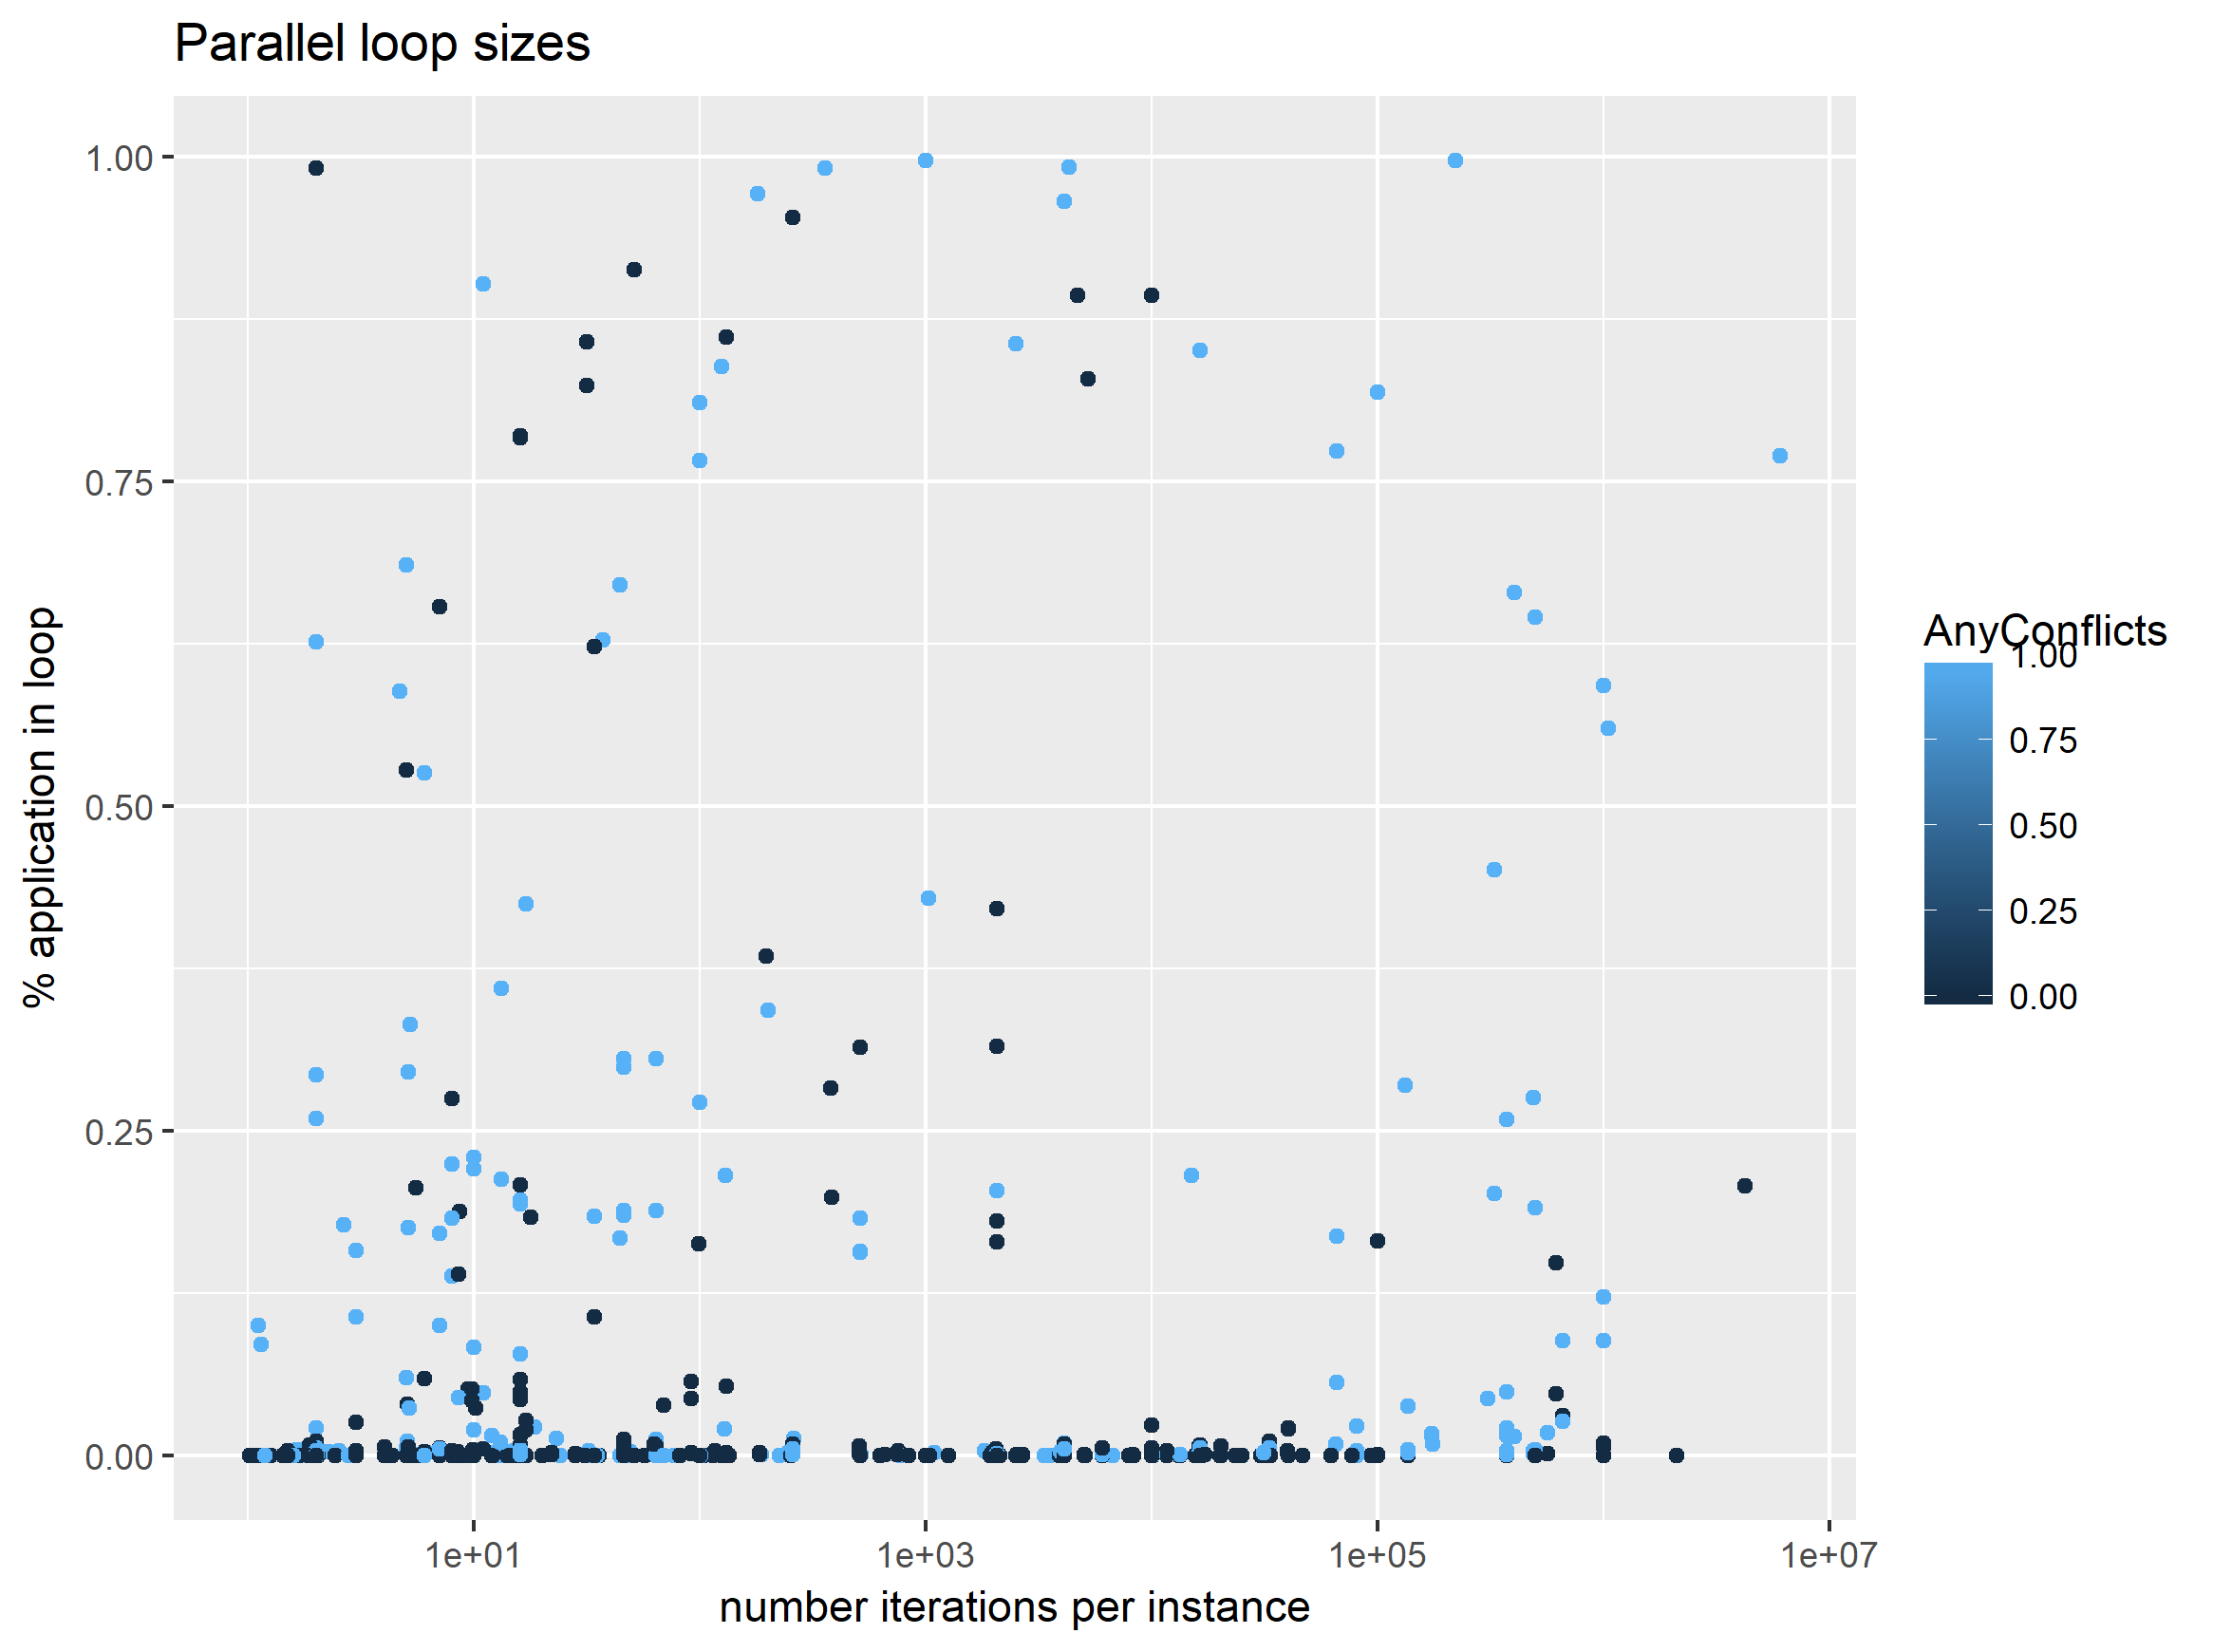
\includegraphics[scale=0.7]{plots/size_iteration_plot.png}
				{\footnotesize Plotting all loops in all applications, loops have conflicts if any iteration conflicted with any other.\par}
			\end{minipage}
		\end{figure}
		
		This plot shows that there are several loops which can be trivially parallelized for significant application speedup. 
		These are the loops which are parallel (do not have conflicts) and have substantial number of iterations (blue dots, upper right). These can be reported to the programmer as targets of trivial parallelization. 
		
		The important loops that are not parallel (have conflicts) but have a large number of iterations are also important (red dots, upper right). These loops could possibly be parallelized with a reduction or with data synchronization and should be reported to the programmer for further investigation.
		
		The dots in the lower-middle are less important than the ones at the top of the plot, but they can also substantially improve application performance. If several smaller parallel loops are present in an application, then parallelizing each of them could result in similar performance gains to parallelizing a large loop. %, the especially when there are multiple such loops in a application.  
		
		But the dots at the very bottom are unimportant to application performance, and so should be ignored. This eliminates most of the loops from consideration. 75\% of the loops include less than 1\% of the total runtime of their respective application. 
		
		
		\subsubsection{Parallelizability of applications}
		
		The parallelism detection tool will only be useful to programmers if it detects parallelism in a  majority of parallel applications. We evaluate this characteristic of the parallelism tool by checking if at least one important loop in each application we evaluate has a useful degree of parallelism. This is a fair evaluation of the parallelism tool because we already know that the Parsec and Rodinia benchmarks include parallel implementations of all of the applications under consideration.%deally the parallelism tool would find important parallelism in every application. %The Rodinia benchmark suite also includes GPU implementations of all the applications taken from that benchmark suite. %So we know that . because the benchmark suites we chose from already parallelized the applications. Does the tool detect all these applications as having significant potential to parallelize? 
		
		We introduce a metric for the percentage of time spent that can be eliminated from the application by parallelizing the loop. It assumes a sort of idealized parallelism. It is calculated as
		$$\text{time eliminated} = \frac{(\text{instructons executed in loop}) \times \frac{\text{iterations per instance} - 1}{\text{iterations per instance}}}{\text{instructions executed in application}} $$
		%where the loop size is the proportion of time (approximated by instruction count) spent inside the loop. 
		The percent time eliminated term, $\frac{\text{iterations per instance} - 1}{\text{iterations per instance}}$ assumes no overhead, infinite cores, and uniform loop iterations.
		These assumptions are extremely optimistic, and so this estimate of time eliminated may also be overly optimistic. But it gives a rough estimate of parallizabililty. Many of the loops which score highly, are in fact very useful to parallelize, which we know since the benchmark suite successfully parallelized them. The loops which score poorly are certainly not useful to parallelize, as there is little gain found even with these generous assumptions. 
		So this metric can be interpreted as an upper bound on how much the loop can reduce application performance if parallelized. 
		
		%\subsubsection{Substantial parallelism of }
		\begin{figure}
			\caption{Performance improvement by idealized parallelization}%Possible speedups with parallelization}
			\label{fig:application-parr}
			
			\begin{minipage}{0.73\textwidth} % choose width suitably
				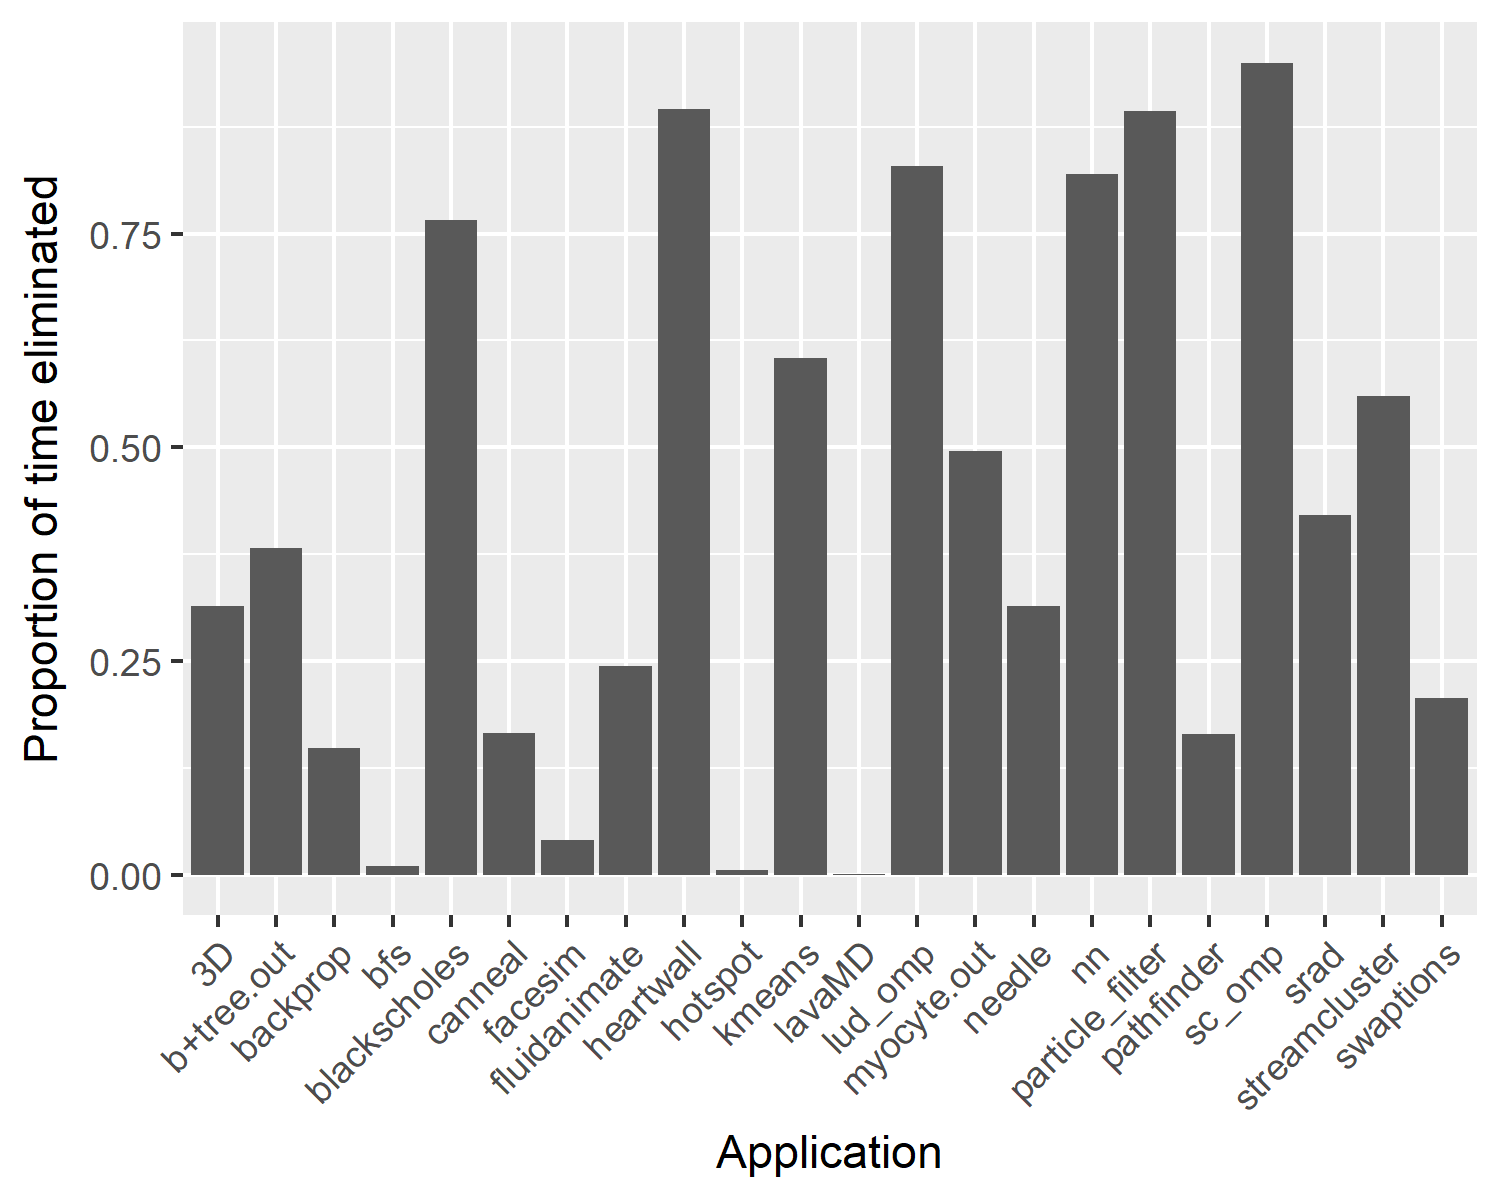
\includegraphics[scale=0.9]{plots/application_idealized_speedup.png}
				{\footnotesize Speedup by parallelizing a the best loop in the given application assuming no overhead and infinite cores.\par}
			\end{minipage}
		\end{figure}
		This estimate of application speedup is a poor indicator of application parallelizability, %and so it is not particularly helpful information to give to a programmer, 
		but it can give us some confidence that the parallelism tool will in fact be somewhat useful for many different applications. 
				
		According to this metric, we detected some substantial parallelism in most of the profiled applications. 
		Figure \ref{fig:application-parr} shows speedup of entire applications assuming idealized parallelization of the loop in the program which results in the greatest time eliminated. \texttt{bfs}, \texttt{hotspot} and \texttt{lavaMD} show little potential for parallelism, as none of the parallel loops are very important to the application. In contrast, \texttt{heartwall}, \texttt{LUD}, and \texttt{blackscholes} show promise for large performance gains by parallelizing a single loop. Others applications are more ambiguous, such as \texttt{swaptions} and \texttt{fluidanimate}, because while parallelizing a single loop cannot increase application performance that much, it is possible that parallelizing several loops can in fact improve performance substantially. Since this plot only gives information about a single loop, it cannot say either way.
		

		\subsubsection{Scale of detected parallelism}
		
		The scale of the parallelism is one of the most important considerations when evaluating what sort of hardware to run the loop on. There are two aspects to scale. 
		
		First, there is the number of threads the work can be divided into. GPUs can run thousands of threads in parallel, while CPUs can at most run a few dozen. Since loop iterations are usually uniform, this can be estimated with the number of iterations in a loop instance. 
		
		Second, there is the amount of work that is done in each thread. Unlike idealized parallelism, real world parallelism on both CPUs and GPUs requires substantial time for the hardware to divide the work into parallel threads at runtime. This means that loops which do little work per iteration and have few iterations may not be effectively divided onto threads on either GPUs or CPUs. 
		Figure \ref{fig:paralleism-scale} plots these two metrics for the important parallel loops in all the applications. 
		
		\begin{figure}
			\caption{Parallelism scale of important parallel loops}
			\label{fig:paralleism-scale}
			
			\begin{minipage}{0.6\textwidth} % choose width suitably
				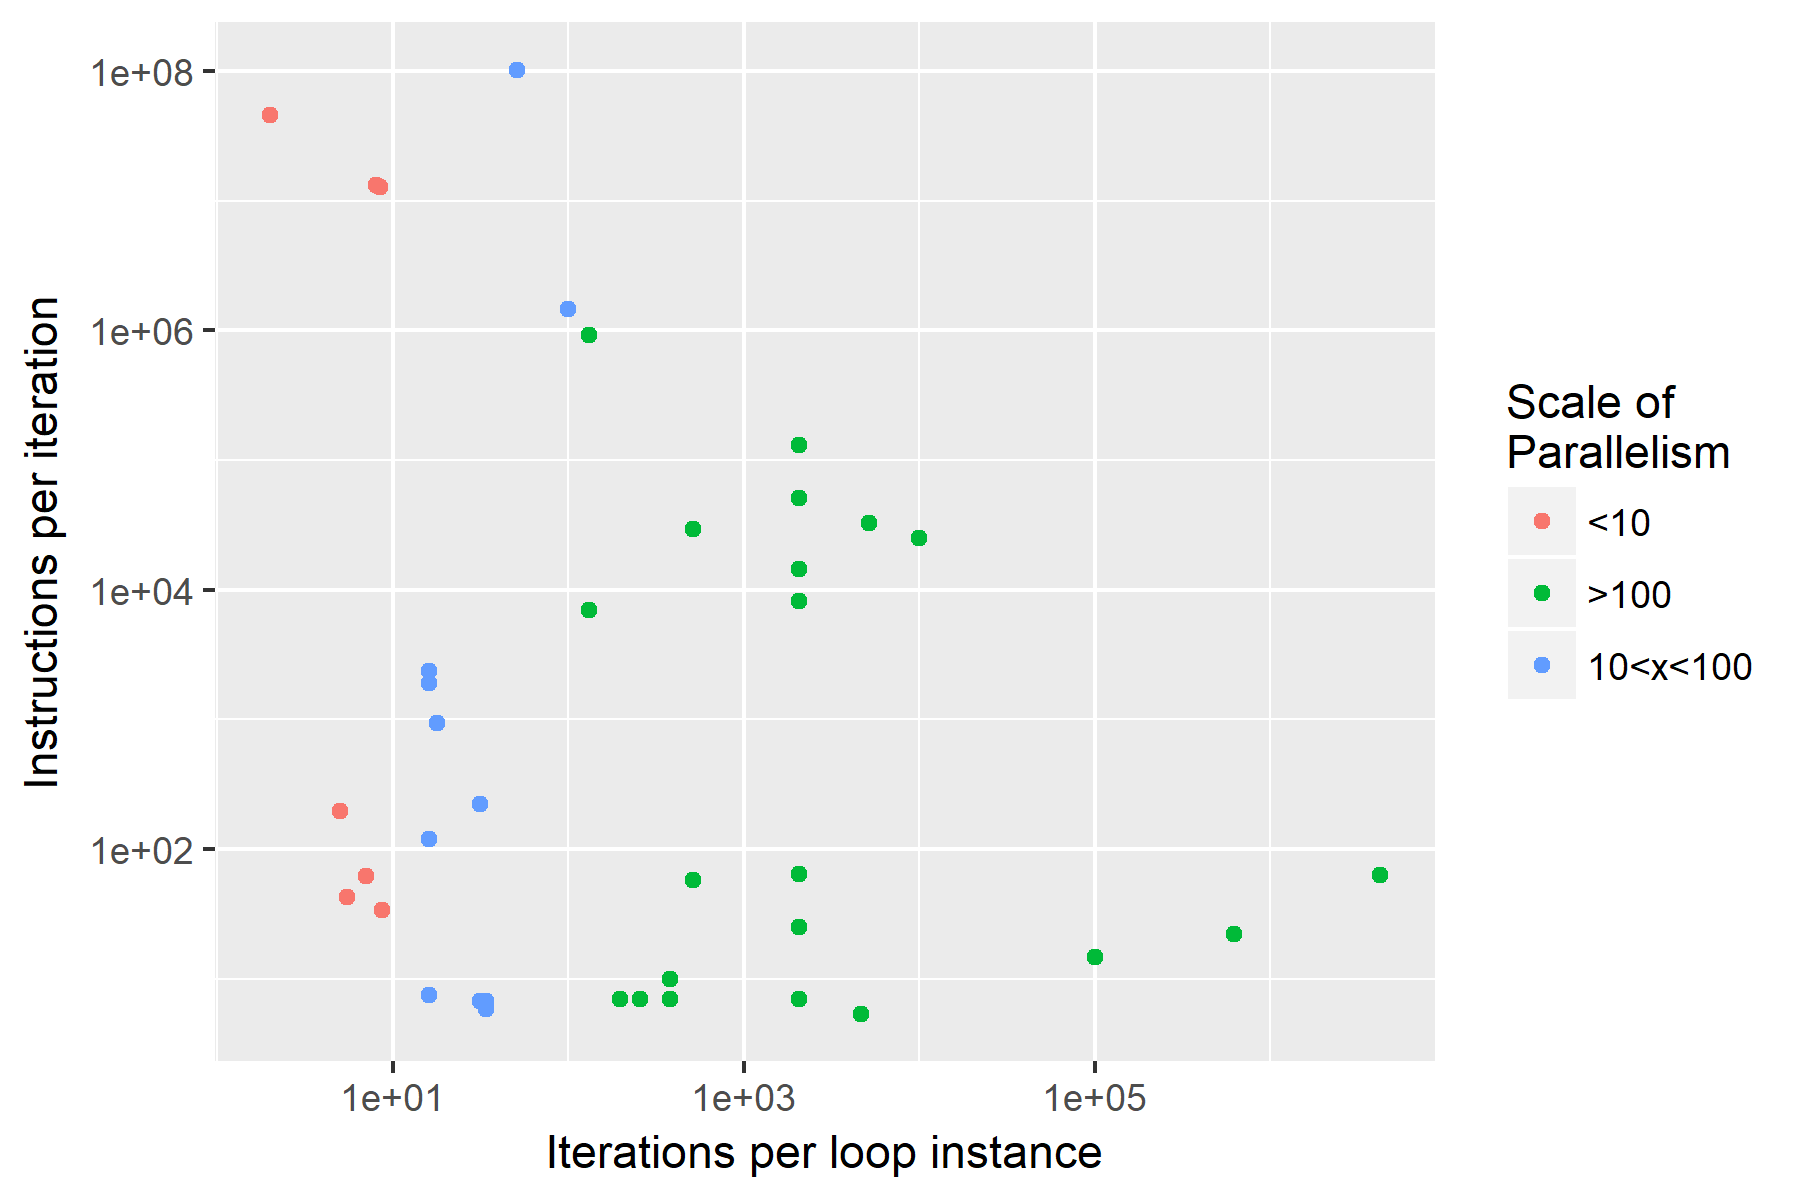
\includegraphics[scale=0.7]{plots/categorized_conflicts.png}
				{\footnotesize Loops which could speed up the program by 10\% or more assuming idealized parallelism. \par}
			\end{minipage}
		\end{figure}
		
		
		CPUs can run a small number of threads effectively, and are ideal for parallelizing loops with a small number of iterations where each iteration does substantial work (upper left, colored red). GPUs are ideal for loops which have a large number of iterations (colored green). Loops which have a middling number of iterations (colored blue), and also have substantial work done per iteration (upper part of the graph), could be parallelized more effectively on a GPU or a CPU depending on additional details of the hardware under consideration. %If the programmer is targeting a server with 32 hardware threads, then that might result in a different evaluation than if the platform is a laptop with 4 hardware threads.%ifFor example in a decision between a laptop with 4 hardware threads and a integrated graphics card with 
		
		%\subsubsection{Questionable parallelizability of some important parallel loops}
		
		However, the loops in the bottom left of Figure \ref{fig:paralleism-scale} may not be parallelizable on hardware because the overhead of distributing iterations of the loop onto either CPU or GPU threads may be greater than the benefit of parallelizing the loop. The parallelism detection tool should inform the programmer about this problem, or the programmer may be misled by the idealized analysis into thinking that the loop would be valuable to parallelize.
		
		%There are types of parallelism which do not involve threads, such as CPU vectorized instruction. There are also optimizations, such as thread pools, which can minimize overhead of thread processing. Finally, sometimes parallelizable nested loops can be combined into a single parallel loop which does more work. But until further investigation, the loops on the bottom left corner of Figure \ref{fig:paralleism-scale} may not be large enough to parallelize. 
		
		%\subsubsection{Scale of parallelism on CPUs vs. GPUs}
		
		
		%CPU threads have substantial overhead: even using optimizations to reduce thread overhead like thread pools, it is not always beneficial to parallelize loops with little work in the inside of the loop, such as the loops near the bottom and left of the plot. 
		
		
		%It will be used only to eliminate loops which score poorly from consideration. This will eliminate the many small loops with little importance to the program, and also loops which are not detected to be parallelizable. 
		
		%, or loops with . Loops which score low on this metric will not be useful to parallelize, loops that score high are not necessarily good candidates for parallelization. 
		
		
		
		%first cutlook at how 
		
		%These assumptions can certainly lead to misleading results, it sometimes corresponds to actual parallelization.

		
		\subsubsection{Uniformity of useful parallel loops}
		
		It greatly simplifies analysis to assume that important parallel loops are uniform, i.e., all the loop iterations do the same amount of work. Notably, this assumption was utilized in our analysis of parallelizability of applications and scale of parallelism. While this is true for many loops, some loops have substantial variability in iteration length that can impact analysis of parallelizability as well as the type of parallel architecture the loop is most suited for. 
			
		To see why this is a problem, consider the idealized parallel machine where an infinite number of threads can run in parallel. Consider a loop with 1000 iterations that can run in parallel, but one of those loop iterations takes as much time all the others combined. In this case, overall loop performance can at most be doubled, since the one iteration takes up half of the sequential time. But if you assume uniformity of iterations, then performance would be calculated to increase by 1000 times, so the actual and predicted speedup would be off by a factor of 500. %In real massively parallel machines, this problem can be even worse, since each thread of a massively parallel machine like a GPU is typically slower than a thread of a CPU. So a parallel version of a loop could potentially run much slower than a sequential one. 
		%So non-uniform loops have serious implications to parallelizability. %This is even more important in the case of massively parallel hardware, like GPUs, since each thread is slower than a GPU thread. 
		
		Luckily, for the applications we examined, most loops are roughly uniform. Figure \ref{fig:uniformity-tail-etc} shows a metric of uniformity plotted over the number of iterations per loop instance. The metric chosen is the maximum iteration length over the mean length. Only loops which could speed up the program by 10\% or more assuming idealized parallelism are shown. 
		
		The two dots in the top left of the graph are loops which have serious problems for parallelizability. They only have 10 loop iterations each on average, but the maximum iteration length is 10 times the mean iteration length. This means that performance may not be increased substantially by parallelization, since a single iteration dominates the runtime of the loop. 
		
		The loop that appears in the top right of the graph is not so problematic. After all, it has over 10,000 loop iterations. If the iterations are carefully distributed over threads, it is possible that the variance between iteration lengths would not have a significant impact on performance, since the smaller iterations could be coalesced together into threads comparable in length to the large thread. But since the programmer has to do extra work to accomplish this, the tool should report this non-uniformity to the programmer.
		
		The loops which show moderate amounts of variance need to be similarly evaluated on a case by case basis. For 67\% of the important loops shown, the maximum iteration length is less than 10\% greater than the mean iteration length, so most of the important loops are in fact uniform. 
		
		%So a value of 10 means that the maximum 
		
		%High values indicate some variance in the 
		
		\begin{figure}
			\caption{Uniformity of loop iterations in important parallel loops}
			\label{fig:uniformity-tail-etc}
			
			\begin{minipage}{0.6\textwidth} % choose width suitably
				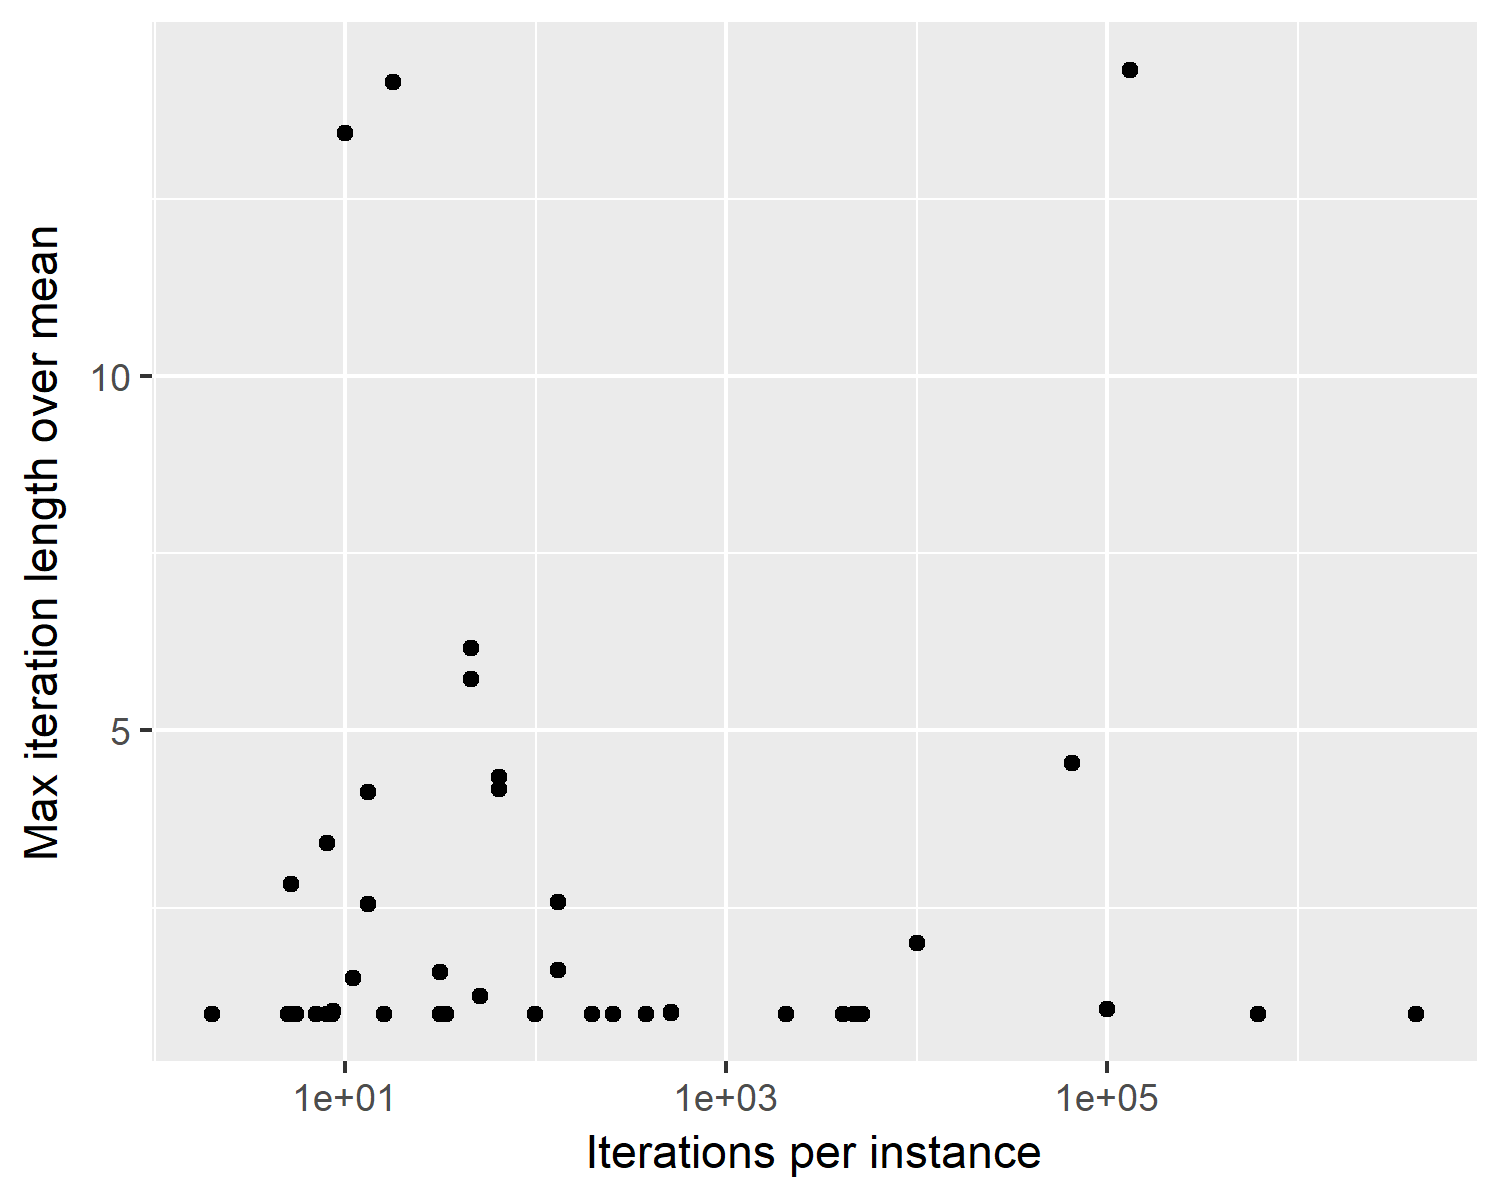
\includegraphics[scale=0.7]{plots/tail_iters.png}
				{\footnotesize Loops which could speed up the program by 10\% or more assuming idealized parallelism. \par}
			\end{minipage}
		\end{figure}
		
		
	\subsection{Future work}
		\label{s:par-fut-work}
		
		This section suggests that this parallelism information can be rather useful to both the programmer and any further characterization of the code. Future work could create a tool which a programmer can easily use to evaluate parallelism. The programmer would provide the inputs to the application, and the analysis tool will tell the programmer where to consider different sorts of parallelism.
		
		A crude version of this tool was implemented to help debug the parallelism detector. It annotates the source code with comments containing the instruction addresses of the loops and with information about conflicts. Code example \ref{ce:par-tool-output} shows an example of this output on some matrix multiplication code. Note that the actual tool outputs more information, and the output is truncated here for better presentation. 
		
		\begin{codeexample}
			\caption{Example output of parallelism tool}
			\label{ce:par-tool-output}
		\begin{verbatim}
		const int size = 100;
		int * A = random_array(size*size);
		int * B = random_array(size*size);
		int * C = random_array(size*size);
		//LOOP 4006b9: ConflictedIterations: 0 TotalLoopIterations: 101
		for(int i = 0; i < size; i++){
		    //LOOP 4006ca: ConflictedIterations: 0 TotalLoopIterations: 10100 
		    for(int j = 0; j < size; j++){
		        //LOOP 4006db: ConflictedIterations: 990000
		        //TotalLoopIterations: 1010000
		        for(int k = 0; k < size; k++){
		            //PARALLEL_CONFLICT FOR 4006db: LaterPC: 400701
		            //EarlierPC: 400760 NumConflictIters: 990000
		            C[i*size+j] += B[i*size+k] * A[k*size+j];
		        }
		    }
		}
		\end{verbatim}
		\end{codeexample}
	
		In its current form, a developer can use this tool to find parallel loops, and see how many iterations they run in. For example, the outer loop of the matrix multiplication has 0 conflicting iterations, which means it is parallelizable. This can help assure the programmer that parallelizing the loop is possible. 
		%If the programmer also knows that parallelizing it would improve performance
		
		For loops which have conflicts, the developer can track down where these conflicts are in the source code. In this case, the inner loop has a conflict. This conflict is labeled by the loop identifier so the programmer can easily track down which conflicts match with which loop. %be found in a large codebase because the conflict is labeled by the loop identifier. 
		 
		Future work could improve the tool by:
		
		\begin{itemize}
			\item Adding more useful information about the loops such as the length and variance of their iterations. This should help the programmer evaluate whether the loops would be profitable to parallelize.
			\item Summarizing the important parallel and possibly parallel loops to investigate further. This may be important for a programmer to navigate large codebases with hundreds of loops. 
			%\item Making the output more user friendly
			%\item Making the vague observations in this section about scale of parallelism and variability of loops into precise metrics that could be easily used. 
			\item  Add an overall score of GPU and CPU parallelism for each loop, perhaps with some kind of performance modeling. 
			\item  Adding static analysis that detects register and stack dependencies as discussed in  section \ref{s:stack-reg-con}.
		\end{itemize} 
	
	\section{Matching parallelism with other metrics}
	
		One goal of this thesis is to try to characterize programs that are effective on CPUs vs. GPUs. But as discussed in Section \ref{s:workload-characht}, choosing the right hardware requires investigating other program metrics than just the scale of parallelism. GPUs and CPUs have all sorts of different hardware characteristics which significantly affect the viability of running certain loops on them. %including parallelism models which treat branches differently, memory models which give different importance to predictable memory, and more. 
		To capture some of these differences we collected the metrics described in Table \ref{table:metric-names} for each loop.
		
		
		\begin{table}
			\caption{Other metrics collected}
			\label{table:metric-names}
			\begin{tabular}{ |p{4.5cm}|p{9.6cm}| }
				\hline
				Metric name & Metric description \\
				\hline \hline
				SwitchesOverBranches & Number of time a branch path changes direction over the number of times a branch instruction is executed \\ \hline
				SwitchesOverInstructions & Number of time a branch path changes direction over the number of instructions executed \\ \hline
				PercNonStridedAccesses & Percentage of accesses which do not access memory as a stride \\ \hline
				StridedAccessesBelow16 & Percentage of accesses which are strides of length 16 bytes or less \\ \hline
				StridedAccessesAbove16 &  Percentage of accesses which are strides of length 16 bytes or more \\ \hline
				PercFixedAccesses & Percentage of accesses which are strides of length zero, i.e. they access the same location of memory location repeatedly \\ \hline
				MemoryAccessesPerInstr & Number of memory accesses over number of instructions \\ \hline
				PercAccessesReads & Percentage of memory accesses which are reads  \\ \hline
			\end{tabular}
		\end{table}
		
		\subsubsection{Variability of metrics in important parallel loops}
		
		These metrics will only be important in predicting overall performance if they are not consistent across all the loops. Figure \ref{fig:other-metrics} tries to capture single variable variance by showing how all the important parallel loops score on the different metrics. 
		To interpret the importance of this figure, take the StridedAccessesAbove16 boxplot as an example. This boxplot shows three loops where over 50\% of accesses are strided accesses where the stride length is over 16 bytes. The rest of the loops are shown to have less than 20\% of this type of access. The significant difference between these groups of loops may have hardware implications that we can exploit to improve performance prediction.
		The most important takeaway of this plot is that it does suggest that there is substantial variance within each of these metrics. 
		While this does not capture overall variance of these performance characteristics, it is a first cut on whether these metrics may turn out to be useful. 
		
		%Each boxplot is a proportion, but the different boxplots are not directly comparable. The fact that SwitchesOverInstructions only has low values is not concerning because even having 2\% of instructions be diverging branches may have serious implications for performance on GPUs. 
		
		%Figure \ref{fig:other-metrics} does suggest that there is substantial variance within each of these metrics. For example, 
		
		\begin{figure}
			\caption{Other metrics of important parallel loops}
			\label{fig:other-metrics}
			
			\begin{minipage}{0.6\textwidth} % choose width suitably
				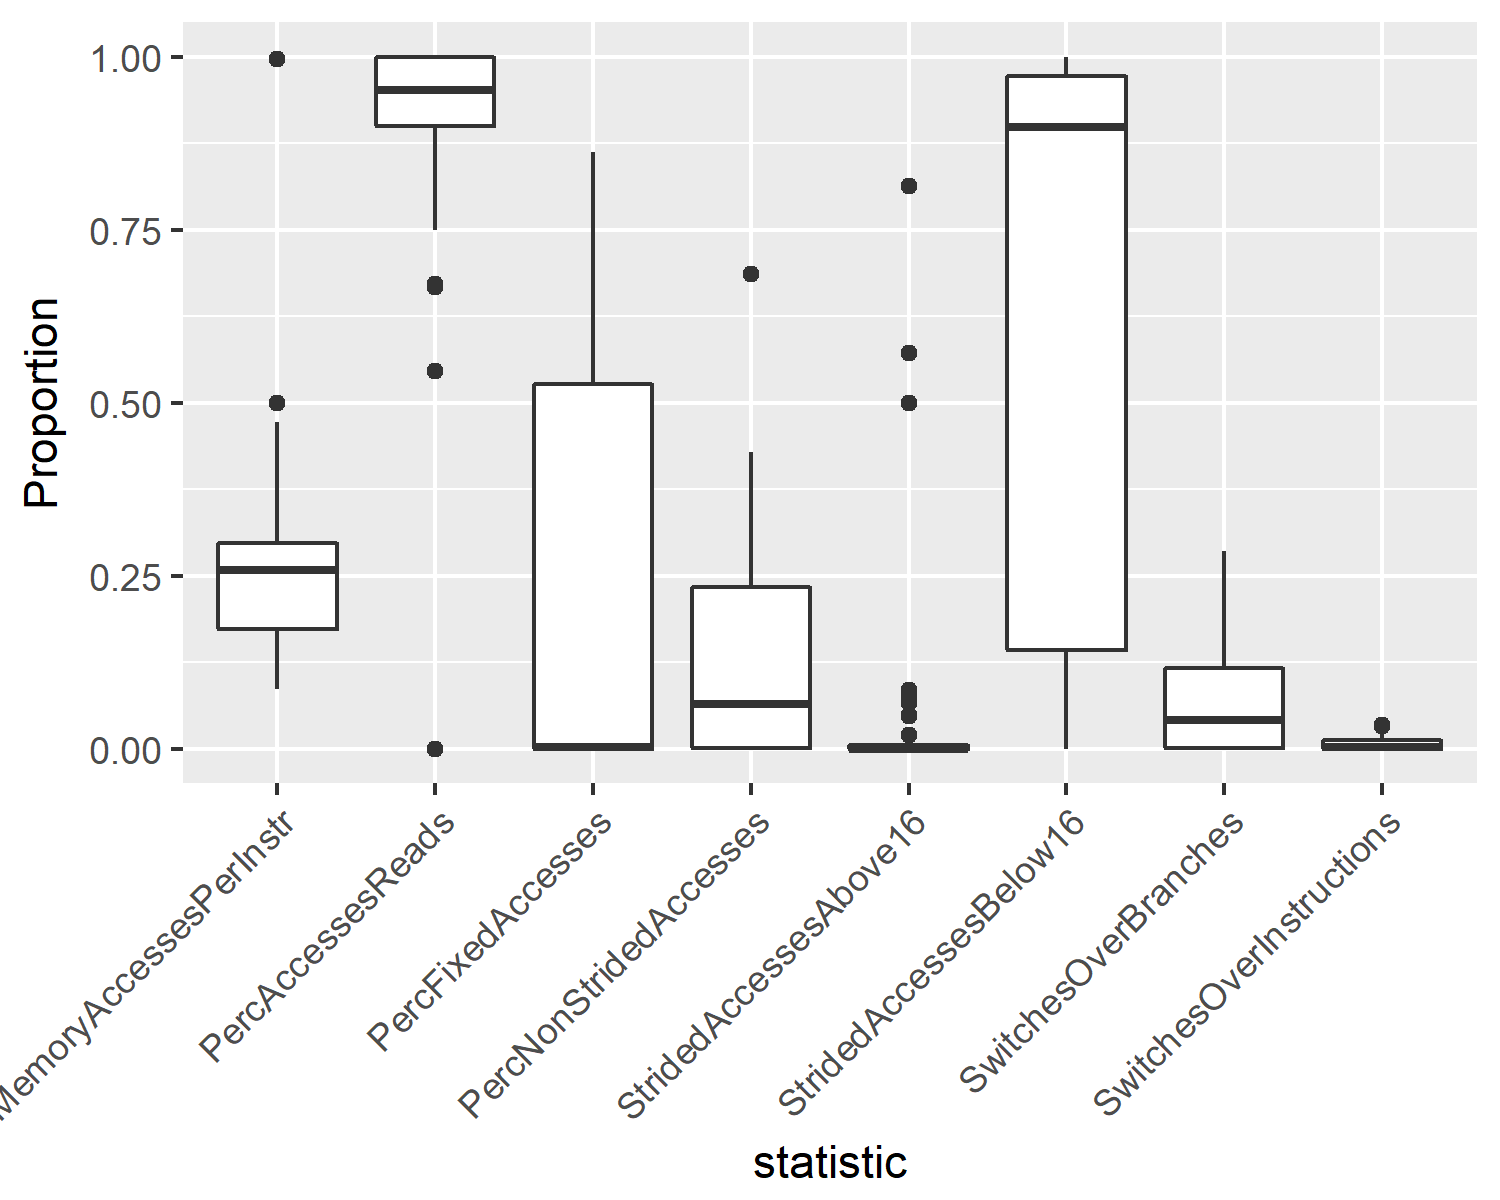
\includegraphics[scale=0.7]{plots/stats_variablility_plot.png}
				{\footnotesize Loops which could speed up the program by 10\% or more assuming idealized parallelism \par}
			\end{minipage}
		\end{figure}
	
		\subsection{Future work}
		
		Unfortunately, due to time restrictions, we were not able to use the metrics to evaluate loop performance on different hardware. Future work would combine metrics similar to these with parallelism summaries discussed in Section \ref{s:important-paralleism} and build a predictive performance model which would indicate to a programmer if and how to parallelize the loop. Such information could be displayed to the programmer by a tool like is described in Section \ref{s:par-fut-work}.

\chapter*{Conclusion}
         \addcontentsline{toc}{chapter}{Conclusion}
	\chaptermark{Conclusion}
	\markboth{Conclusion}{Conclusion}
	\setcounter{chapter}{4}
	\setcounter{section}{0}

	This thesis set out to create a tool that helps programmers understand how their code might best utilize heterogeneous computing. It addresses several challenges involved with completing this goal and leaves other challenges open for future work. %a first step towards this goal by creating a tool which evaluates loop level parallelism. Our efforts solved some 
	
	One of the problems encountered by prior work in parallelism detection is the massive memory overhead of the naive algorithm.
	We confirmed that the simplest implementation uses too much memory to run real applications on real systems, and implemented two methods for reducing the memory footprint: stride compression and bit compression. We found that these two methods use comparable magnitudes of memory on most of the applications examined, and both are vast improvements over the naive method. As programmers find new ways of making use of larger quantities of system memory, these techniques will not be good enough, so we hint that future work could combine bit and stride compression into a single tool. 
	
	Another potential problem with the naive method of parallelism detection is that it only finds a certain type of parallelism: trivial loop-level parallelism. This raises the question of whether it is useful in detecting parallelism that is actually important to program performance. We found evidence that it does detect important parallelism for most the applications studied. To the extent to which the applications we examined are representative, this tool does in fact detect real parallelism. 
	Future work could make the tool more accessible to the programmer by producing more informative output. Future work could also produce more accurate results by incorporating static analysis. 
	
	Finally, we started addressing the challenge of how to inform the programmer about software characteristics other than parallelism and their effects on hardware performance. We collected several loop level metrics other than parallelism, and suggested that they would be important in evaluating the effectiveness of accelerating the loops on GPUs vs. CPUs. 
	Future work can determine how to pair those metrics with parallelism, how to interpret or model them in a way that has direct implications for performance, and evaluate if different metrics are needed. Future work could also evaluate new metrics for hardware platforms other than CPUs and GPUs.
	
	If all these challenges are addressed, and a quality tool is produced, then programmers who use the tool should be much more able to evaluate what kind of parallelism, if any, is appropriate for different parts of their code. This will allow them to make more informed decisions about investing time to adapt the code to work on heterogeneous hardware. %working on those systems.
	
	%the metrics be paired with parallelism information somehow. 
	
	
	%The most important aspect of heterogeneous computing is the importance placed on parallelism
	%
	%a tool that 
	%We built a %memory efficient parallelism detector, and found that it is useful in detecting important parallelism on real applications. We identified some possible metrics that could potentially 



%This is where endnotes are supposed to go, if you have them.
%I have no idea how endnotes work with LaTeX.

  \backmatter % backmatter makes the index and bibliography appear properly in the t.o.c...

% if you're using bibtex, the next line forces every entry in the bibtex file to be included
% in your bibliography, regardless of whether or not you've cited it in the thesis.
    \nocite{*}

% Rename my bibliography to be called "Works Cited" and not "References" or ``Bibliography''
% \renewcommand{\bibname}{Works Cited}

%    \bibliographystyle{bsts/mla-good} % there are a variety of styles available;
%  \bibliographystyle{plainnat}
% replace ``plainnat'' with the style of choice. You can refer to files in the bsts or APA
% subfolder, e.g.
 \bibliographystyle{APA/apa-good}  % or
 \bibliography{thesis}
 % Comment the above two lines and uncomment the next line to use biblatex-chicago.
 %\printbibliography[heading=bibintoc]

% Finally, an index would go here... but it is also optional.
\end{document}
